\section{Results}
\label{sec:results}
To test the filters' ability to increase general robustness of a high-order solver, we have implemented their formulation in \gls{hf} for triangular elements and performed simulations where the solver would become unstable otherwise. In addition, we analyze the impact the filters have on a well-resolved 2-D simulation.

We wanted to test the increase of robustness in extreme cases of grid coarseness, high Reynolds number, very low \gls{ma}, and moderate \gls{ma}. It is important to keep in mind that in these cases we are not seeking very accurate results, but rather robustness under all conditions. In order to popularize high-order methods, we need to make them as robust as their low-order counterparts while retaining their benefit of higher accuracy with less computational and setup effort.

The goal is to have a cheap stabilization strategy that preserves boundary conditions for cases in which the mesh is not necessarily perfectly appropriate for resolving the flow physics over the entire domain. This scenario arises frequently in industrial applications, where the mesh would be properly refined at regions of interest and coarse in regions that the engineer/scientist has decided are not as important for the problem at hand.

All the simulations that follow were performed using \gls{hf}\cite{lopez2014verification}. 2-D \gls{ns} equations are being solved, with varying values of \gls{ma}, \gls{re}, time-step ($\Delta t$), and filtering frequency. The common parameters are:
\begin{enumerate}[1.]
\item Four-stage, five-step, low-storage Runge-Kutta time-stepping method (\gls{rk45}) \cite{carpenter1994fourth} was used in the \gls{gpu}s, and forward Euler was used when running a simulation in CPUs
\item Polynomial solution representation ($p$) of order $4$. Rusanov Flux as a Riemann solver, and a \gls{ldg}~\cite{cockburn1998local} viscous flux.
\item Filters with width $h = 10$ and weighting parameter $\alpha = 0.8$.
\item Starting from uniform flow
\item Characteristic boundary conditions at the inflow and outflow. No-slip, isothermal wall boundary conditions at the cylinder's surface.
\item All quantities non-dimensionalized with free-stream temperature and cylinder wall temperature of $300$, reference length of $1$.
\item Flow properties: $\gamma = 1.4$, Prandtl number $\mathrm{Pr} = 0.72$, gas constant $R = 286.9 \frac{J}{Kg K}$, viscosity determined by Sutherland's law with reference temperature of $291.15 K$ and reference viscosity of $\mu = 1.827\mathrm{e}-5$
\end{enumerate}

Results of interest are shown in Table \ref{table:results}. Accuracy of the results is not expected. Nevertheless, as a reference, for the flow around a cylinder at \gls{re}$= 1e6$, $\bar{C_D} \approx 0.6$ in~\cite{achenbach1968distribution}, $\bar{C_D} \approx 0.4$ in \cite{roshko1961experiments} and $\St \approx  0.4$ in \cite{roshko1961experiments}. It is important to note that at a high \gls{re}, flow over a cylinder can result in a range of $\bar{C_D}$ and $\St$ values, as the results become highly sensitive to surface roughness and the level of free-stream turbulence~\cite{zdravkovich1997flow}. The experimental values of $\bar{C_D}$ vary from 0.17 to 0.40, and those of $\St$ from 0.18 to 0.50.

Because of the results obtained in Case 4, it is good to keep in mind that for flow around a cylinder at \gls{re}$\approx 2e2$, $\bar{C_D} \approx 1.18$ in \cite{roshko1961experiments} and $\St \approx  0.2$ in \cite{roshko1961experiments}. 


\begin{table}
%\begin{adjustwidth}{-2.1cm}{}
%    \centering
    \cellspacebottomlimit=5pt
    \cellspacetoplimit=5pt
%      \begin{center}                % keep track of old \tabcolsep
        \setlength{\oldtabcolsep}{\tabcolsep}     % 6.0pt
        \setlength{\tabcolsep}{0pt}               % so coloring doesn't run off
                                                  % ends of the table
        \renewcommand{\arraystretch}{2}         % because math expressions
                                                  % almost run into each other

\def \spacing {0.4cm}
\hspace{-2.5cm}
\begin{tabular}{c <{\hspace{\len}}c <{\hspace{\spacing}} 
c <{\hspace{\spacing}}
c<{\hspace{\spacing}} c<{\hspace{\spacing}} c<{\hspace{\spacing}} c<{\hspace{\spacing}} c<{\hspace{\spacing}} c <{\hspace{\spacing}} c <{\hspace{\spacing}} c}
          \toprule
Case & $\Ma$  & $\Delta t$ & $n_F$ & $\bar{C_D}$  &  $\mathrm{St}$ & \specialcell[b]{Flow time \vspace{-0.2cm}\\(s)} & Time steps  & \specialcell[b]{Wall time \vspace{-0.2cm}\\(hours)}& \specialcell[b]{Computing \vspace{-0.2cm}\\ Resources}\\
          \specialrule{\lightrulewidth}{0pt}{0pt} % so row-coloring aligns

1 & $0.2$ &  $5e-5$ &$1000$ &$0.9256$ & $0.1600$ & $1.2069$ &$1,675,700$ & $12.65$&  1 4-core i7 CPU \\
2 & $0.077$ & $5e-5$ &$1000$ & $0.9314$ & $0.1627$ & $15.44$ & $8,252,500$ & $11.78$ & 1 \gls{gpu}\\
3 & $0.87$ & $5e-5$ &$100$ & $1.8383$ & $0^*$ & $1.3833$ & $8,355,256$ & $12.63$ & 1 \gls{gpu}\\
4 & $0.0077$ & $1.25e-5$ &$1000$ & $ 1.18$ & $0.20$ & $53.44$ & $11,428,000$ & $59.51$ & 2 \gls{gpu}s\\

          \bottomrule
        \end{tabular}

      \caption{Summary of simulation results. All cases were run at $\Re = 1e6$ with polynomial representation of order $4$. Cases 1-3 were run using the mesh shown in Figure \ref{fig:meshes}. Case 4 was run using the mesh shown in Figure \ref{fig:meshes2}. Cases with $0^*$ Strouhal number reached an artificial steady-state.}
      \label{table:results}
%      \end{adjustwidth}
    \end{table}


\subsection{Stabilization Strategy}
In the simulations presented here, the solution inside every element in the entire domain is being filtered using Equation \ref{eqn:filter_form} every $n_F$ time-steps, where $n_F$ is an integer to be determined. No sensor is being used to detect problems in the flow.

The frequency of filter application is being chosen in the following heuristic way:
\begin{enumerate}[1.]
\item \label{item:start}Start the simulation with a specific time step and no filtering. Record at what time-step the simulation ends prematurely (produces Nan values) and note the value of the residuals at the last valid time-step.  This step usually takes no more than 1 minute.
\item \label{item:halve_dt}To ensure the simulation is ending prematurely because of grid resolution problems or presence of sharp gradients, and not because of an unstable time step, halve the time step and run the simulation again.
\item \label{item:check_res} Wait for the simulation to exit prematurely. If the residual at this last exit is close in value to the previous exiting residual, the time step in Step \ref{item:halve_dt} was stable. Set the new time step to the time step in \ref{item:halve_dt}. Otherwise, record the exiting residual and go back to Step \ref{item:halve_dt}.
\item Now that a stable time step has been found, apply the filter to the simulation every $n_F$ time steps, where $n_F$ is about $90\%$ of the number of imte-steps it took the simulation to become unstable when unfiltered.
\end{enumerate}

It would certainly be desirable to filter the solution at elements where a problem is detected. Nevertheless, this heuristic approach has so far enabled the stabilization of every case tried and de-couples the effectiveness of the filters from possible shortcomings of aliasing/shock sensors.

\subsection{Coarse mesh used in simulations}
In these tests, we have used the very coarse triangular mesh with $714$ elements shown in Figure \ref{fig:meshes}. The boundary layer is purposefully not resolved properly, as we would like to induce aliasing errors in the unfiltered calculation.

\begin{figure*}
\hspace{-1cm}
\subfloat[Full mesh view \label{fig:mesh}]{%
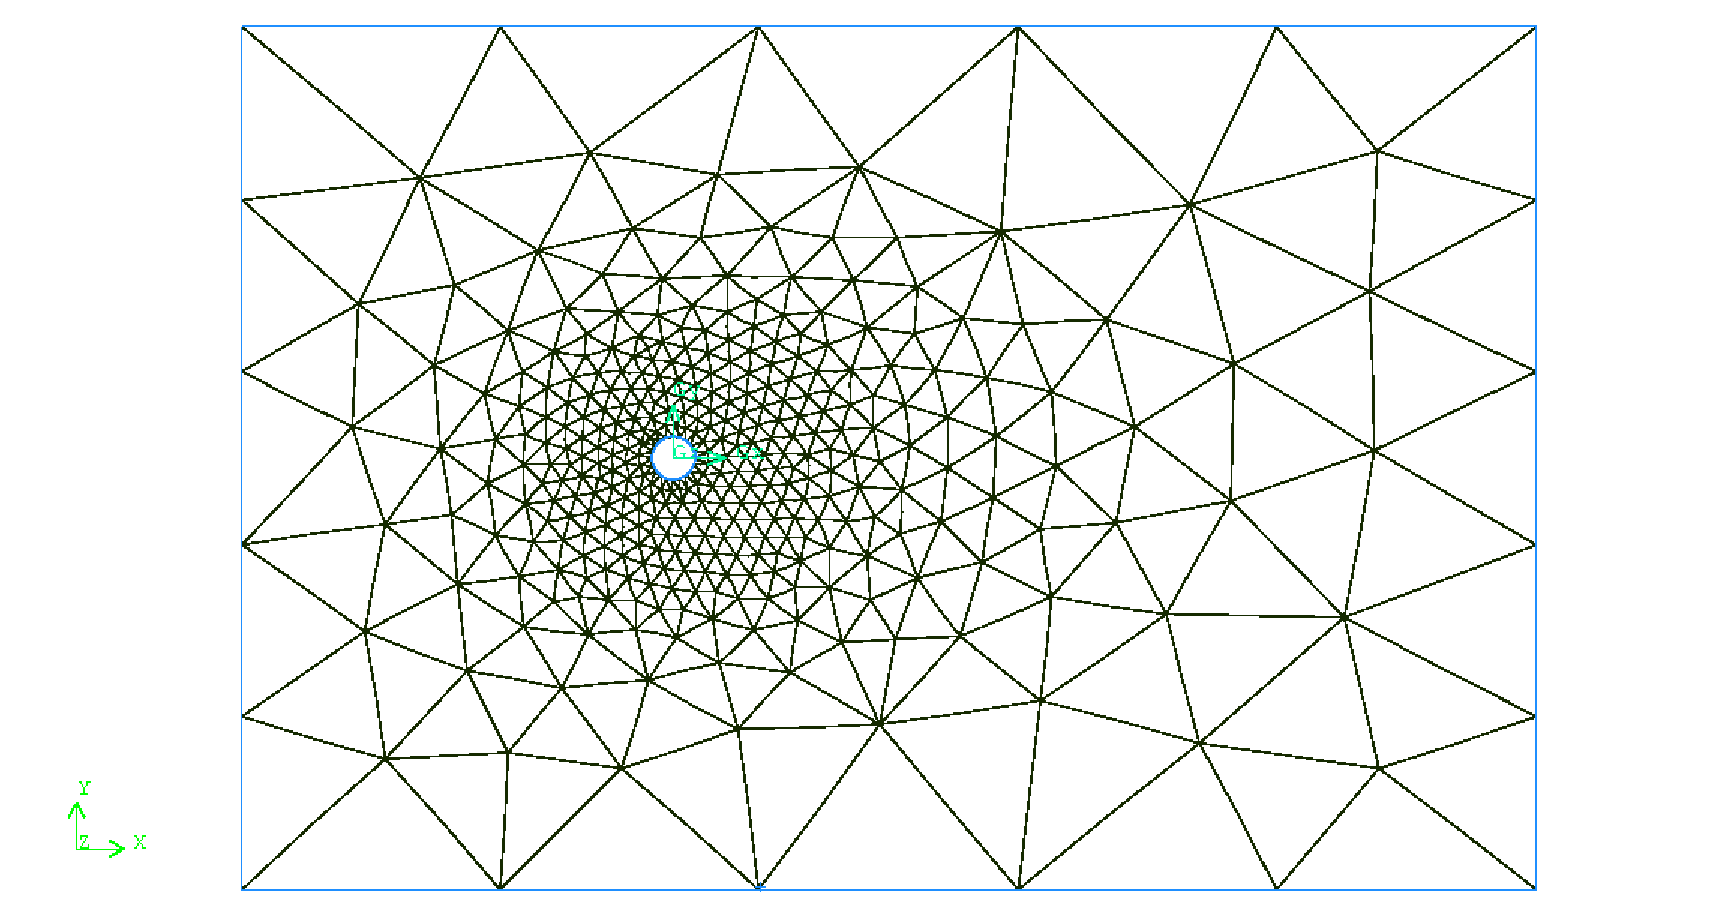
\includegraphics[width=0.55\textwidth]{\lfsdir/figs/MESH2.eps}
}
\hfill
\subfloat[Close-up view \label{fig:mesh_close}]{%
\centering
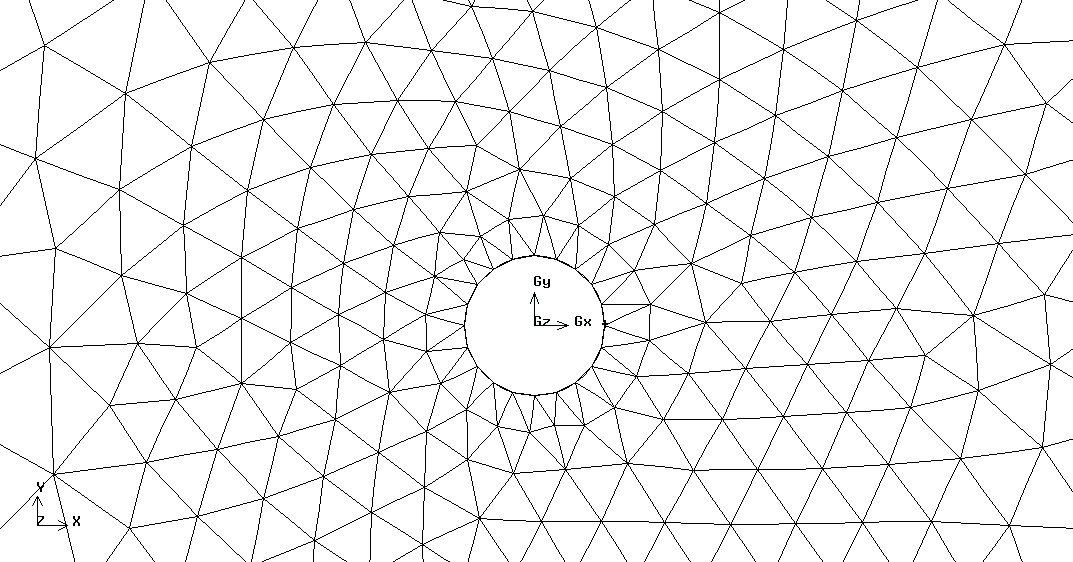
\includegraphics[width=0.55\textwidth]{\lfsdir/figs/MESH_CLOSE.png}
}
\caption{Unstructured, coarse mesh of a circular cylinder with $714$ triangular elements. Elements adjacent to the cylinder have quadratic edges.}
\label{fig:meshes}

\end{figure*}

\subsection{Flow Around a Circular Cylinder, $\bf Re =  10^6, Ma = 0.2$}
This was the first simulation performed after implementing the filters in \gls{hf}, so the \gls{gpu} implementation was not available then. The time-stepping scheme used here is simply forward Euler.

Figure \ref{fig:Ma0.2Re1e6_Ma} shows ``pretty pictures" resulting from the simulation. A video of this simulation is linked \href{https://youtu.be/b6kx8-jrK6Q}{here}.

It is interesting to note that there is a very dissipative form of vortex shedding occurring. The wake region is long, as in lower \gls{re}-number cases.

The simulation remained stable throughout and no human intervention was performed while it was occurring, from the start in uniform flow to the moment it was stopped.

From this experiment, it is unclear what portion of the numerical dissipation arises from the coarse discretization and what portion is due to the filtering operation.

This case demonstrates that the stabilization strategy can work well in cases where the mesh is improperly refined: they stabilize the solution and preserve the boundary conditions.

\begin{figure*}
\hspace{-1cm}
\subfloat[Full view \label{fig:Ma0_2Re1e6_Ma_far}]{%
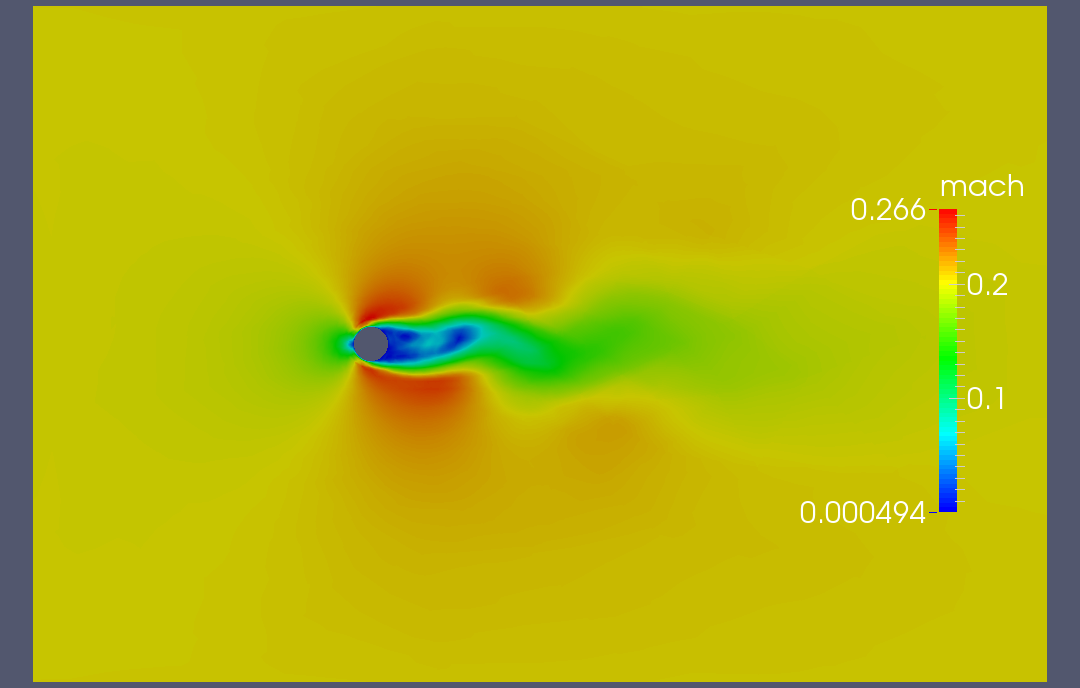
\includegraphics[width=0.55\textwidth]{\lfsdir/figs/Ma0_2--Re1e6_Ma.png}
}
\hfill
\subfloat[Close-up view \label{fig:Ma0_2Re1e6_Ma_close}]{%
\centering
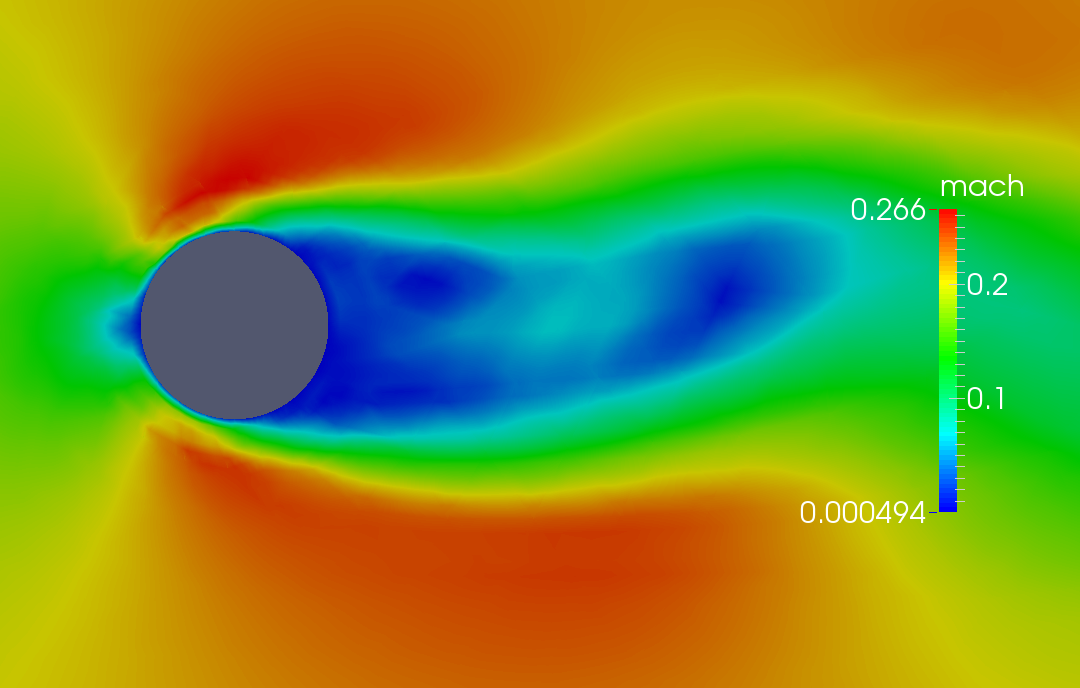
\includegraphics[width=0.55\textwidth]{\lfsdir/figs/Ma0_2--Re1e6_Ma_closeup.png}
}
\caption{Flow past a cylinder. $\Re = 1e6, \Ma = 0.2, p = 4$}
\label{fig:Ma0.2Re1e6_Ma}

\end{figure*}

\subsection{High Reynolds Number, Flow Around a Circular Cylinder, $\bf Re = 10^6, Ma = 0.077$}
This was the first simulation performed using \gls{gpu}s. The lower \gls{ma} case was of interest, as \gls{hf} had not been able to run full simulations of flows with \gls{ma}$< 0.2$.

Figure \ref{fig:Ma0.077Re1e6_Ma} shows the colorful results for this case. Once again, the boundary conditions are satisfied and the simulation is stabilized without further intervention. The same time-step size was used as in the previous case in order to leave as many parameters as possible unchanged.

A video of this simulation is linked \href{https://youtu.be/EymTVFzyPcA}{here} in real-time, and \href{https://youtu.be/8ZH349_GRUA}{here} at 0.1$\times$. A feature of these simulations that can only be appreciated by watching the linked videos is that the filters have a visible effect on the regions where aliasing and instabilities are expected: the rear part of the cylinder and the boundary layer. However, even though the filters are being applied everywhere, smooth, well-resolved regions of the flow look unchanged. To what extent the smooth regions remain unchanged has not been quantified.

\begin{figure*}
\hspace{-1cm}
\subfloat[Full view \label{fig:Ma0_077Re1e6_Ma_far}]{%
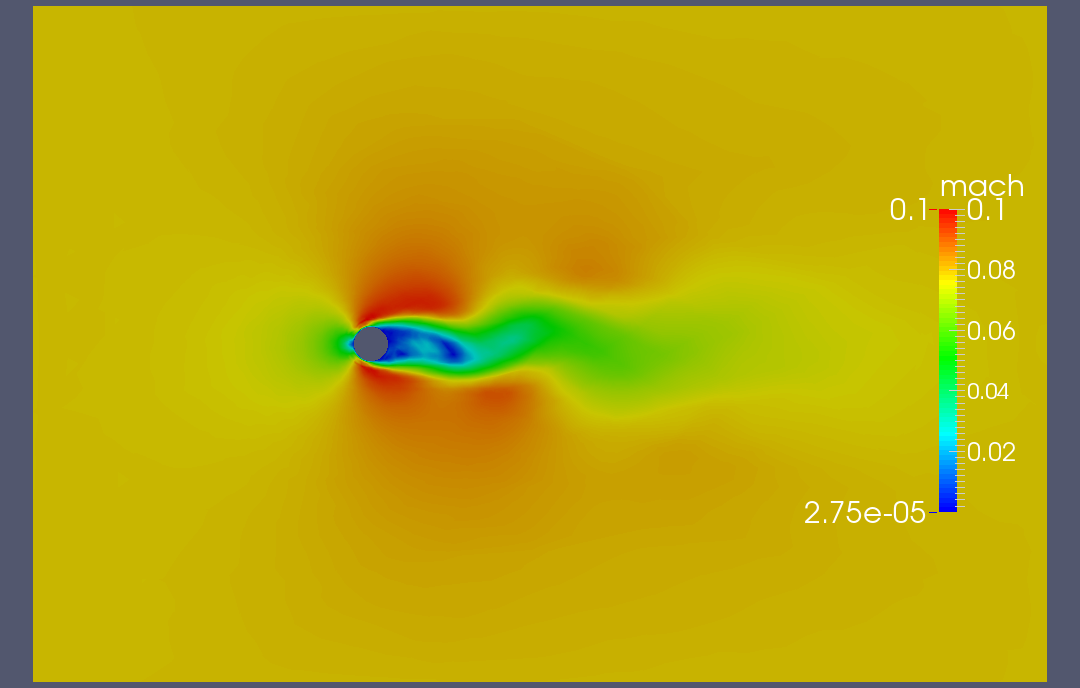
\includegraphics[width=0.55\textwidth]{\lfsdir/figs/Ma0_077--Re1e6_Ma.png}
}
\hfill
\subfloat[Close-up view \label{fig:Ma0_077Re1e6_Ma_close}]{%
\centering
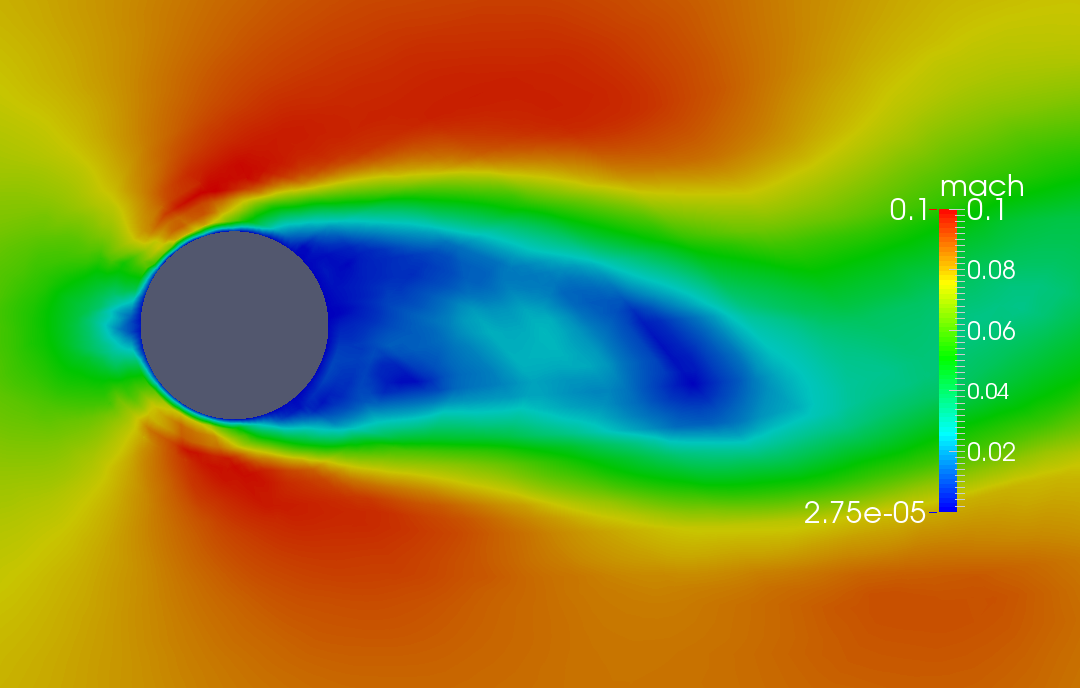
\includegraphics[width=0.55\textwidth]{\lfsdir/figs/Ma0_077--Re1e6_Ma_closeup.png}
}
\caption{Flow past a cylinder. \gls{re}$= 1e6$, \gls{ma} $= 0.077, p = 4$}
\label{fig:Ma0.077Re1e6_Ma}

\end{figure*}

%\subsection{High Reynolds Number, Flow Around a Circular Cylinder, $\bf Re = 10^6, Ma = 0.85$}

\begin{figure*}
\hspace{-1cm}
\subfloat[Full view \label{fig:Ma0_87Re1e6_Ma_unstable_far}]{%
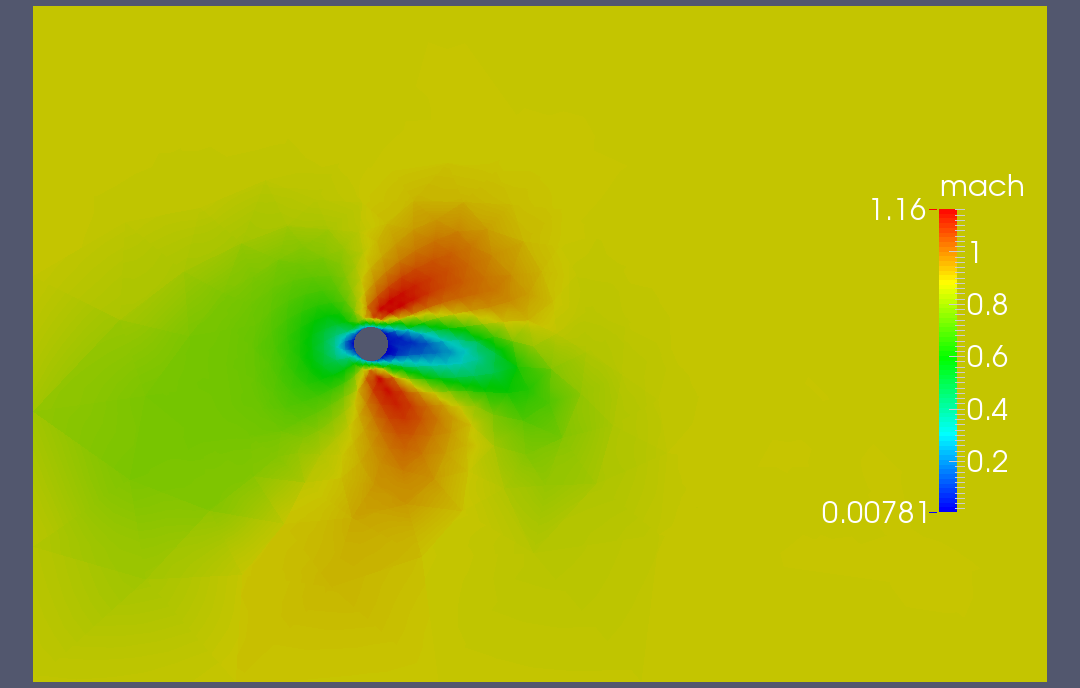
\includegraphics[width=0.55\textwidth]{figs/Ma0_87--Re1e6_Ma.png}
}
\hfill
\subfloat[Close-up view \label{fig:Ma0_87Re1e6_Ma__unstable_close}]{%
\centering
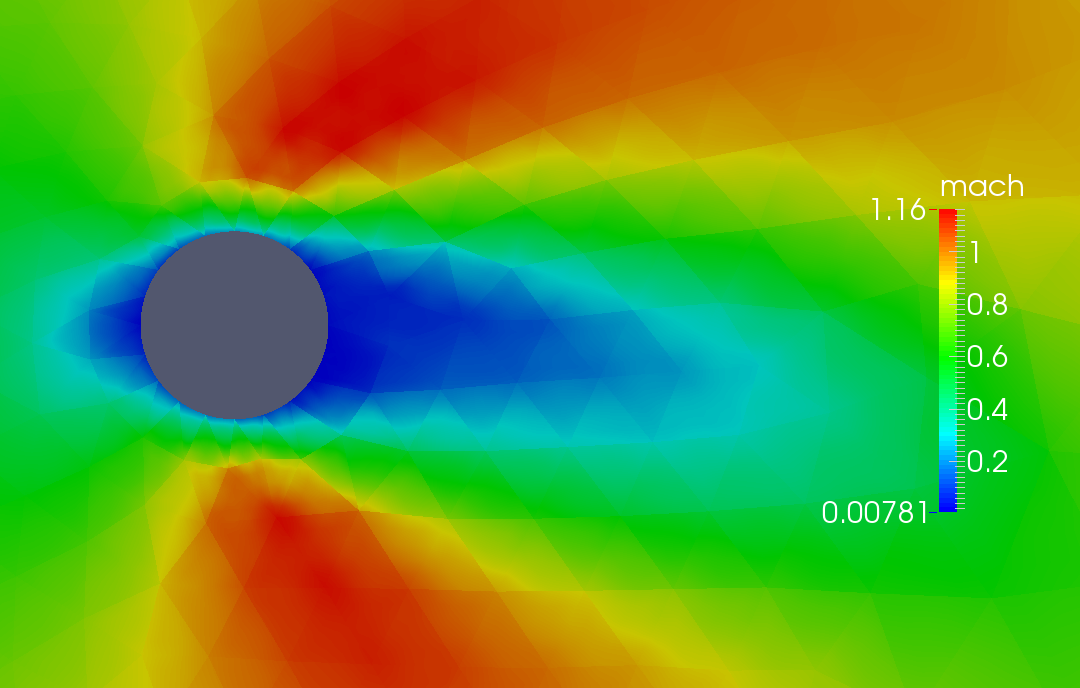
\includegraphics[width=0.55\textwidth]{figs/Ma0_87--Re1e6_Ma_closeup.png}
}

\hspace{-1cm}
\subfloat[Close-up view \label{fig:Ma0_87Re1e6_P__unstable}]{%
\centering
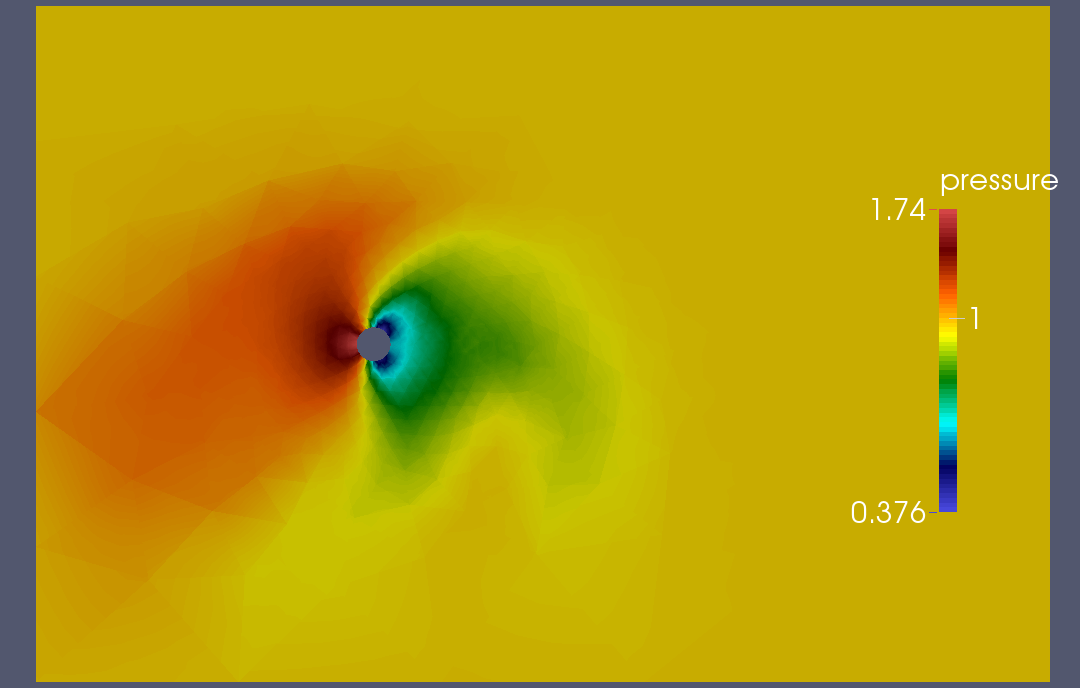
\includegraphics[width=0.55\textwidth]{figs/Ma0_87--Re1e6_P.png}
}
\hfill
\subfloat[Close-up view \label{fig:Ma0_87Re1e6_P__unstable_close}]{%
\centering
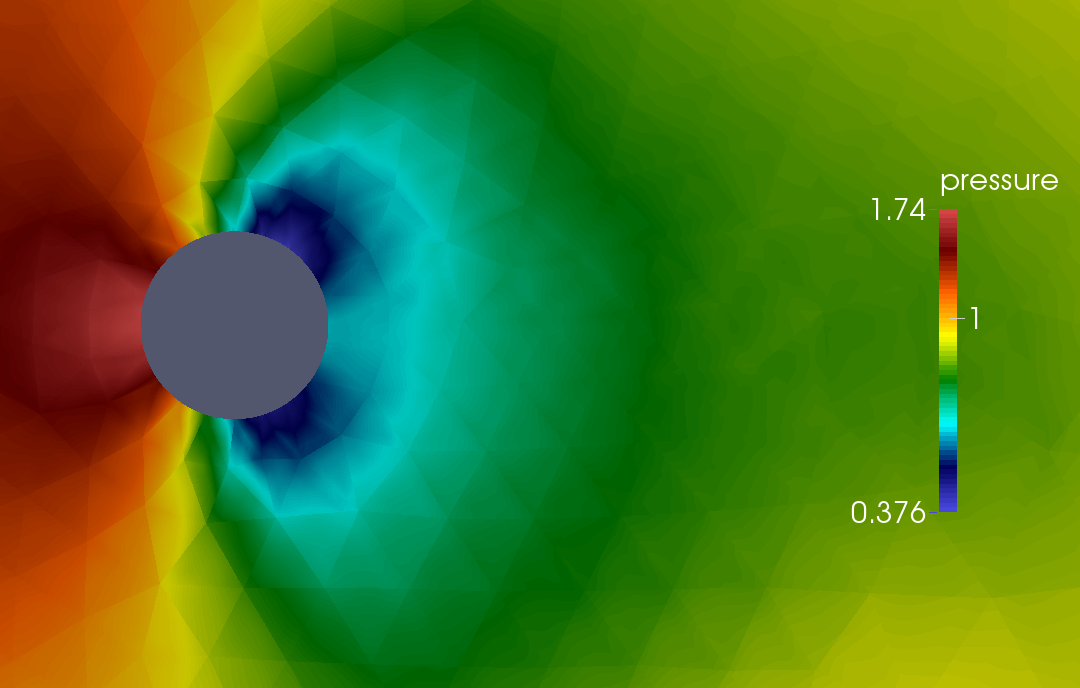
\includegraphics[width=0.55\textwidth]{figs/Ma0_87--Re1e6_P_closeup.png}
}
\caption{$\Re = 1e6, \Ma = 0.87, p = 4$}
\label{fig:Ma0.87Re1e6_unstable_Ma}
\end{figure*}

\subsection{High Reynolds Number, Flow Around a Circular Cylinder, $\bf Re = 10^6, Ma = 0.87$}

This case encompasses all potential sources of instabilities in a high-order solver: poor resolution, aliasing, and sharp gradients. Figure \ref{fig:Ma0.87Re1e6} shows plots of the solution. The simulation shows a clear un-physical asymmetry due to the coarseness of the mesh. Nevertheless, the no-slip boundary conditions are being satisfied and the shock is present. 

Because of the coarseness of the mesh and the high-gradients present in the solution, quite a lot of filtering had to occur. This forced the flow to a ``steady state" and shown in the Residual and $C_D$ plots in Figure \ref{fig:Ma0.87Re1e6_history}.

\begin{figure*}
\hspace{-1cm}
\subfloat[Full view \label{fig:Ma0_87Re1e6_Ma_far}]{%
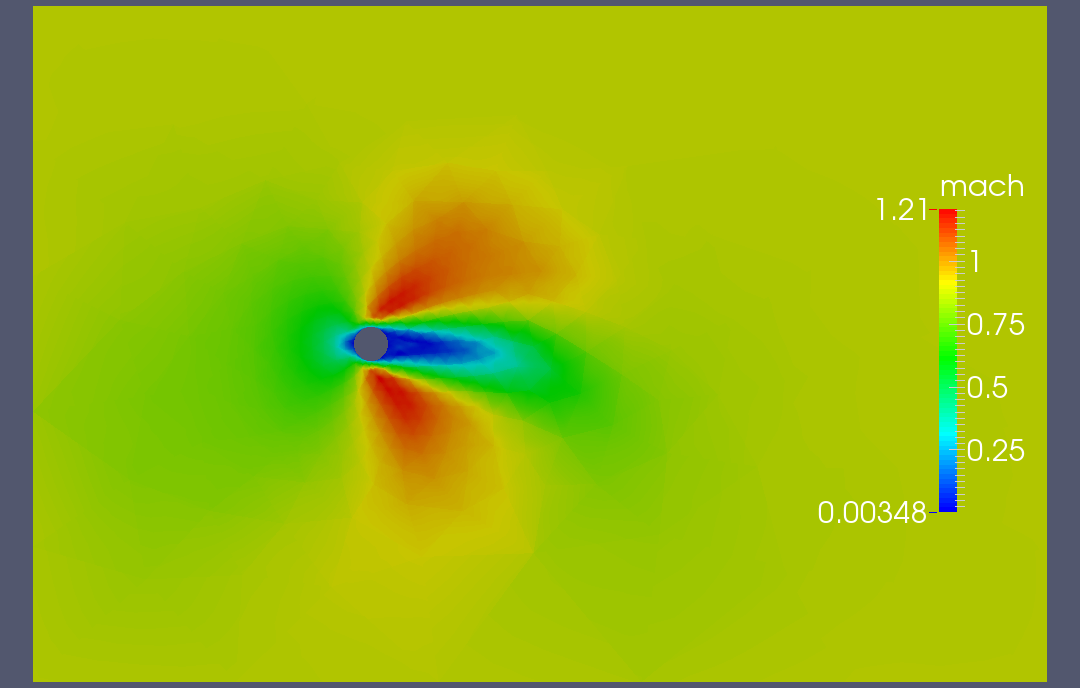
\includegraphics[width=0.55\textwidth]{\lfsdir/figs/Ma0_87--Re1e6_Ma_stable.png}
}
\hfill
\subfloat[Close-up view \label{fig:Ma0_87Re1e6_Ma_close}]{%
\centering
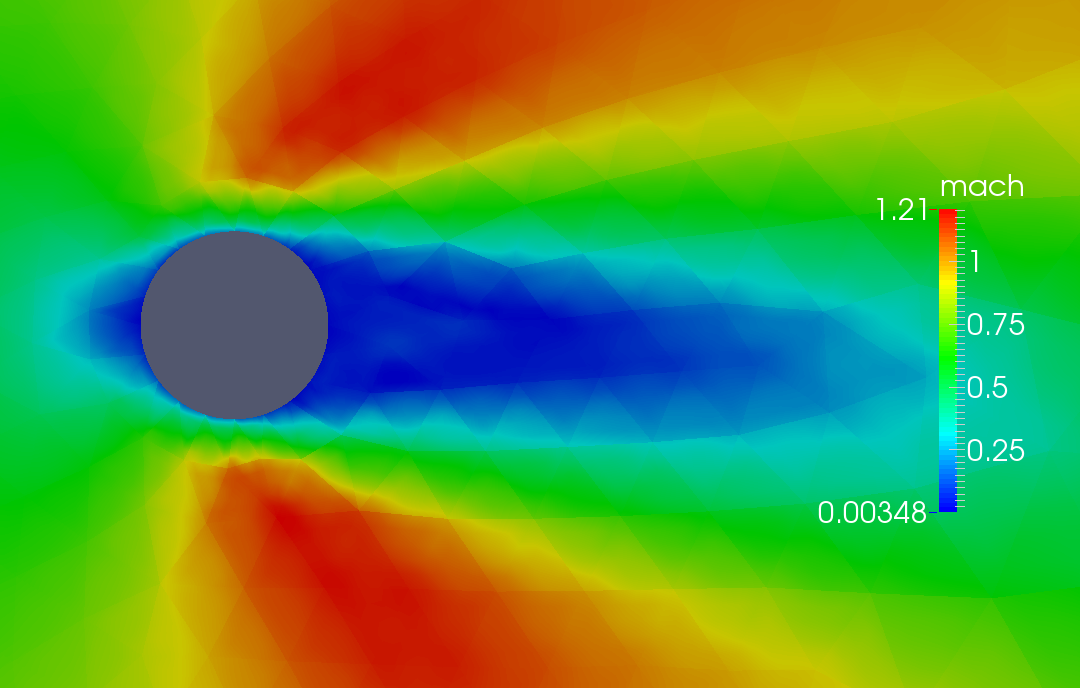
\includegraphics[width=0.55\textwidth]{\lfsdir/figs/Ma0_87--Re1e6_Ma_stable_closeup.png}
}

\hspace{-1cm}
\subfloat[Full view \label{fig:Ma0_87Re1e6_P_stable}]{%
\centering
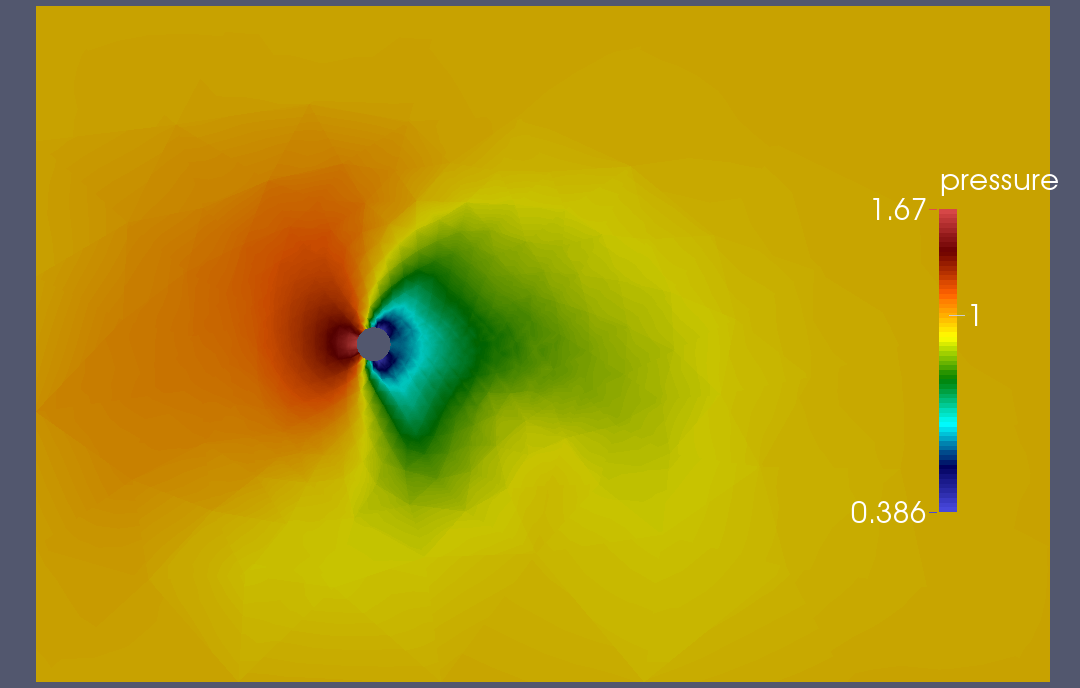
\includegraphics[width=0.55\textwidth]{\lfsdir/figs/Ma0_87--Re1e6_P_stable.png}
}
\hfill
\subfloat[Close-up view \label{fig:Ma0_87Re1e6_P_stable_close}]{%
\centering
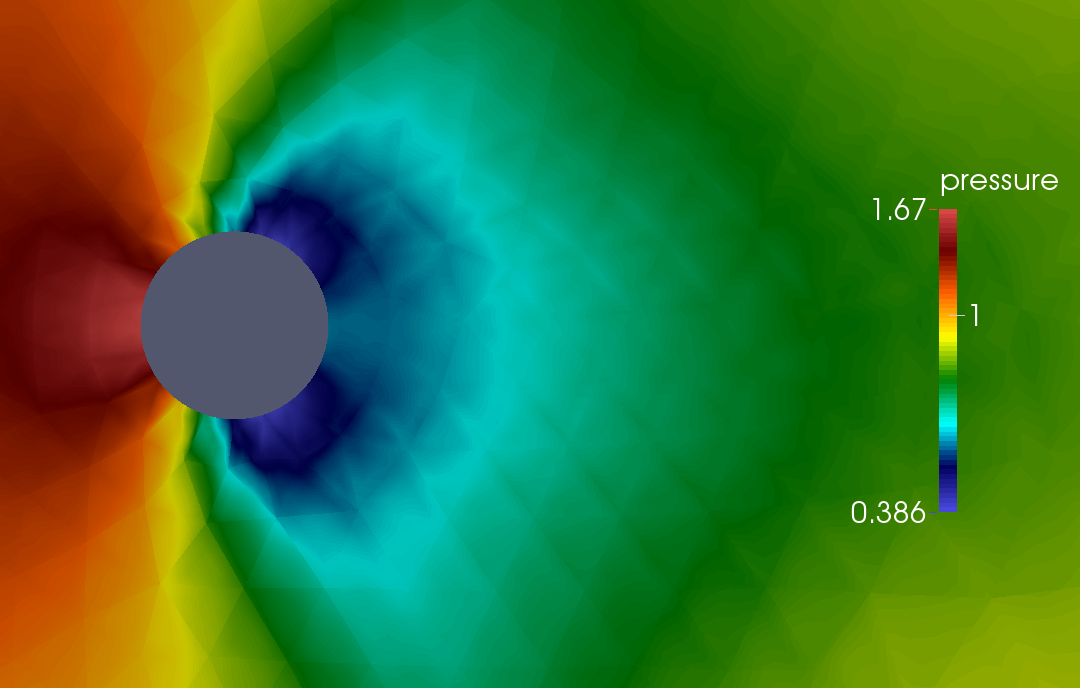
\includegraphics[width=0.55\textwidth]{\lfsdir/figs/Ma0_87--Re1e6_P_stable_closeup.png}
}
\caption{Flow past a cylinder. \gls{re}$= 1e6$, \gls{ma} $= 0.87, p = 4$}
\label{fig:Ma0.87Re1e6}

\end{figure*}

Values of $C_D$ and residual history are shown in Figure \ref{fig:Ma0.87Re1e6_history}. The value of drag ``converges" after time-step $1.846e6$. The residual in the energy conservation equation also ``converges" to a zig-zag pattern after this iteration. Figure \ref{fig:rhoE_res_history} shows the energy residual in the last few thousand time-steps. The sharp decrease in residual magnitude reveals the time-steps at which the filter is being applied.

\begin{figure*}
\subfloat[Drag coefficient history over entire simulation run. ``Steady state" is reached at time-step $1.846e6$. \label{fig:cd_history}]{%
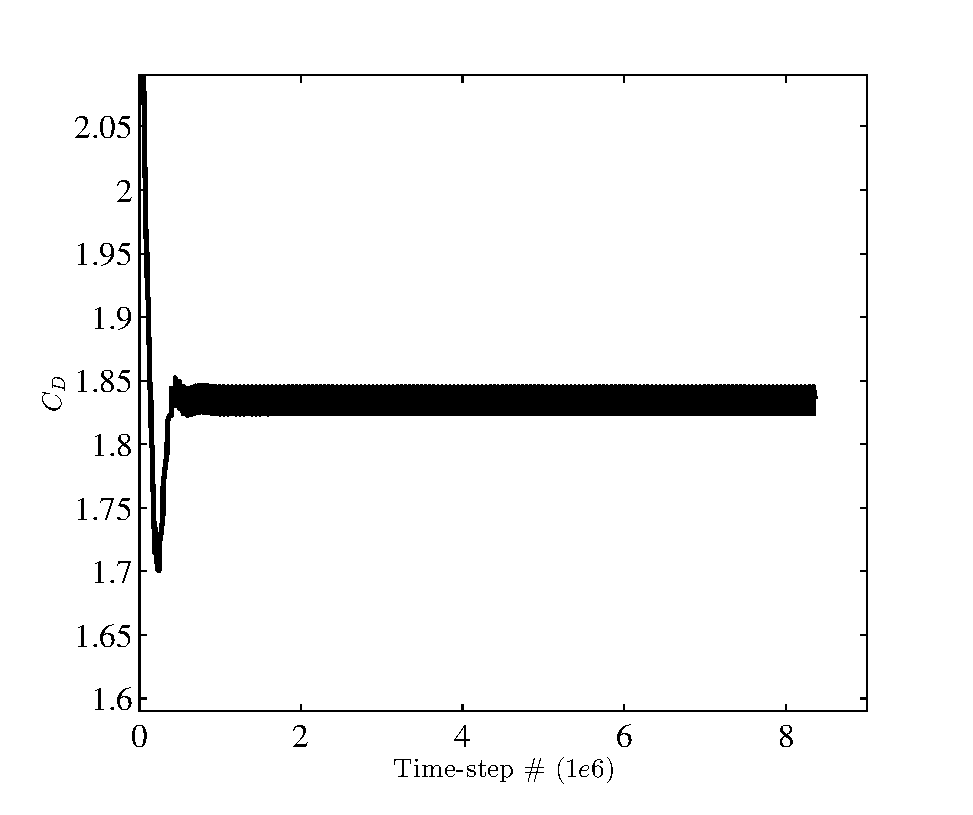
\includegraphics[width=0.55\textwidth]{\lfsdir/figs/unstable_c_d.eps}
}
\hfill
\subfloat[Energy residual history over the last few thousand time-steps \label{fig:rhoE_res_history}]{%
\centering
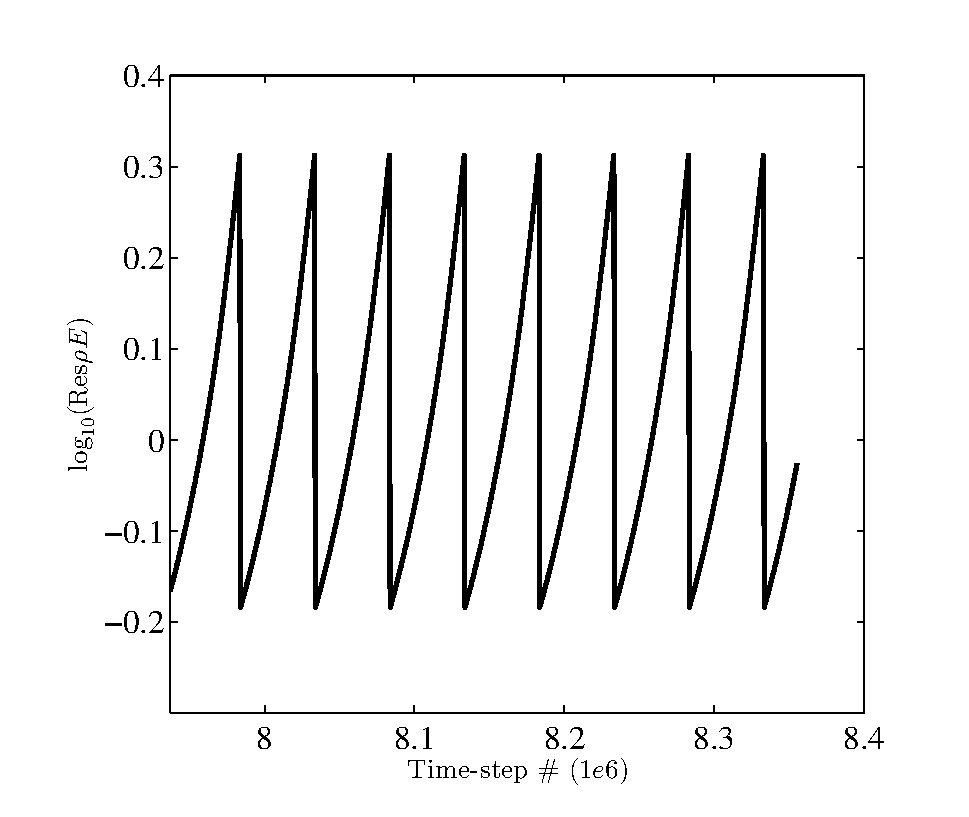
\includegraphics[width=0.55\textwidth]{\lfsdir/figs/unstable_rhoE_res.eps}
}
\caption{History of $C_D$ and energy residual of simulation in Figure \ref{fig:Ma0.87Re1e6}}
\label{fig:Ma0.87Re1e6_history}

\end{figure*}

\subsection{High Reynolds Number, Flow Around a Circular Cylinder, $\bf Re = 10^6, Ma = 0.0077$, less-coarse mesh}
This case was run with the more refined mesh seen in Figure \ref{fig:meshes2}. This mesh is still coarse for standard turbulent computations. It is interesting to note that the predicted $C_D = 1.18$ and $\mathrm{St} = 0.20$ match experimental results for \gls{re}$= 2e2$. This phenomenon could imply that the grid of the stabilized simulation determines the effective Reynolds number being simulated.

A real-time video of this simulation is linked \href{https://youtu.be/XSzWPn2fZ90}{here} for Mach contours, and \href{https://youtu.be/_zIbZgHjepY}{here} for vorticity strength contours. The filters stabilized this almost-incompressible simulation without a problem.


\begin{figure*}
\hspace{-1cm}
\subfloat[Full mesh view \label{fig:mesh2}]{%
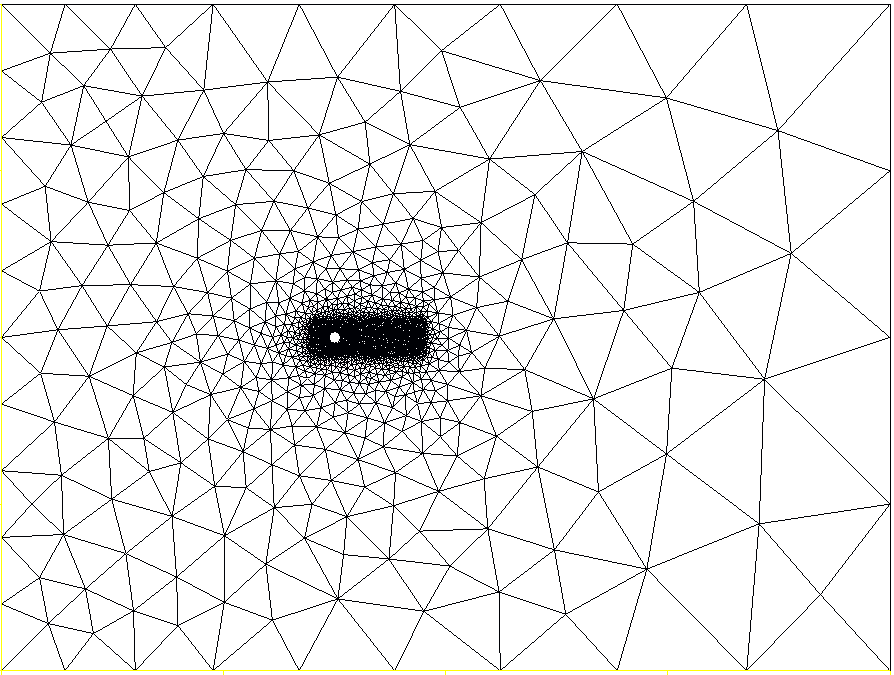
\includegraphics[width=0.55\textwidth]{\lfsdir/figs/cylinder_fine_v2.png}
}
\hfill
\subfloat[Close-up view \label{fig:mesh2_close}]{%
\centering
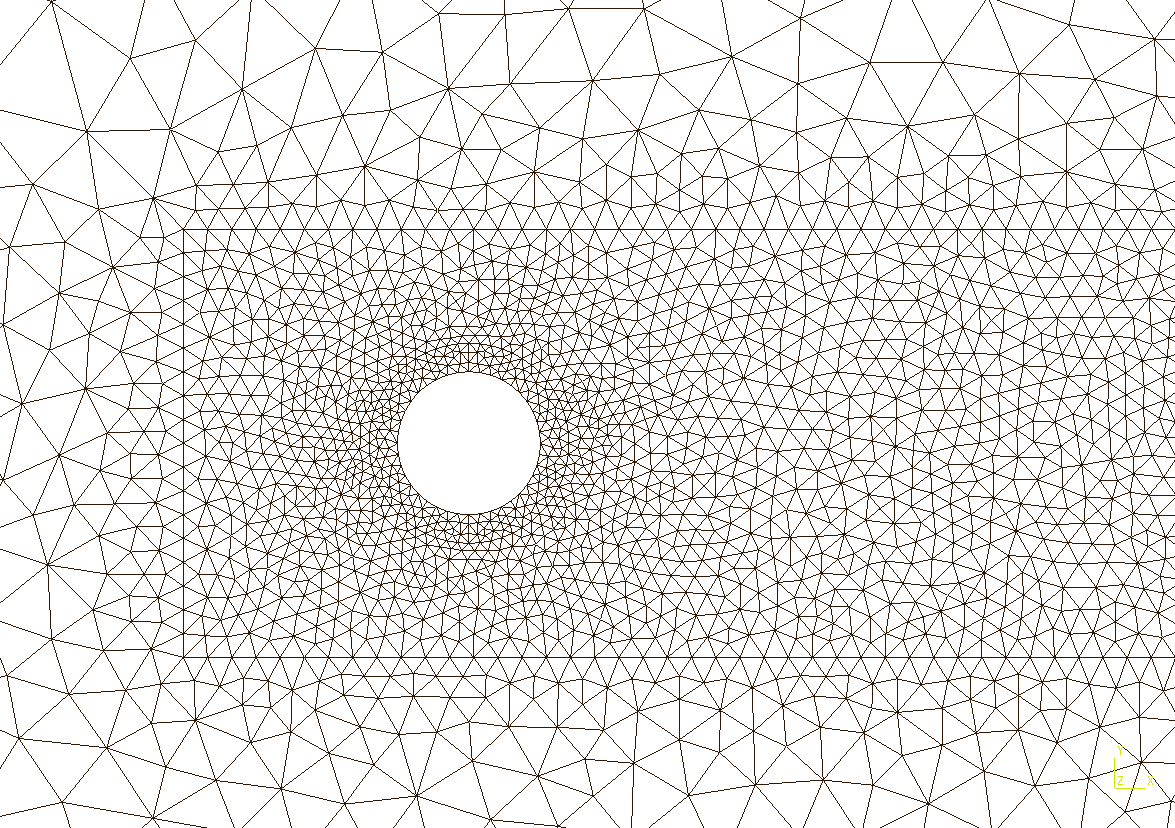
\includegraphics[width=0.55\textwidth]{\lfsdir/figs/mesh_closeup_2.png}
}
\caption{Unstructured, coarse mesh of a circular cylinder with 5,616 triangular elements. Elements adjacent to the cylinder have quadratic edges.}
\label{fig:meshes2}

\end{figure*}


\begin{figure*}
\hspace{-1cm}
\subfloat[Full view \label{fig:Ma0_0077Re1e6_Ma_far}]{%
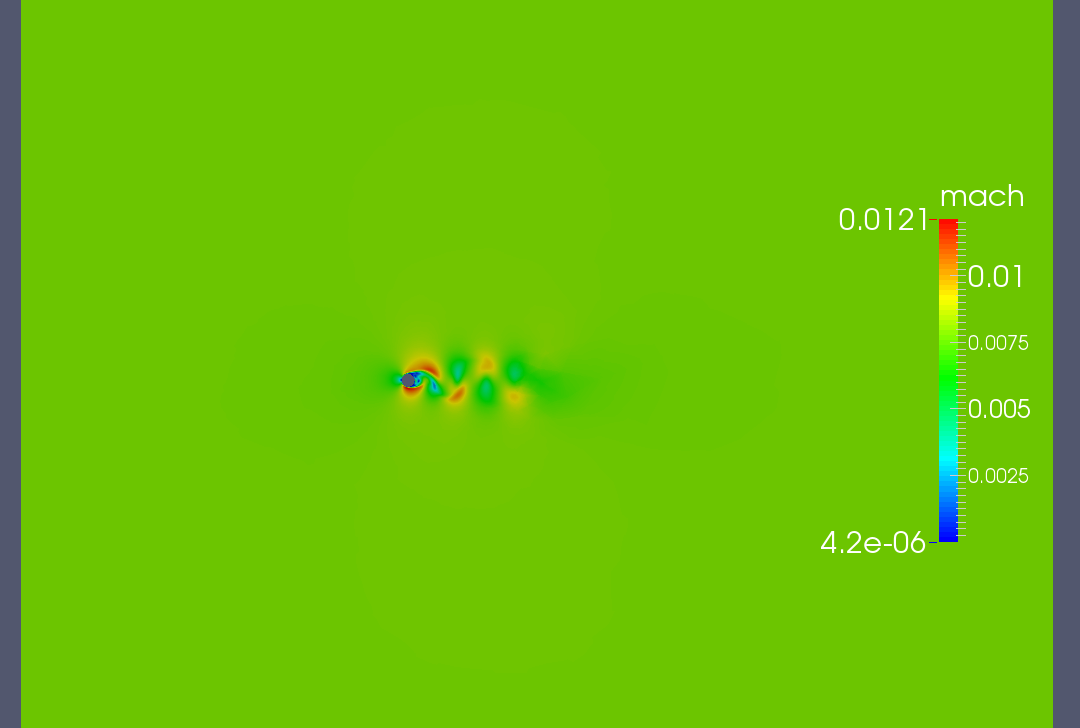
\includegraphics[width=0.55\textwidth]{\lfsdir/figs/Ma0_0077--Re1e6_Ma.png}
}
\hfill
\subfloat[Close-up view \label{fig:Ma0_0077Re1e6_Ma_close}]{%
\centering
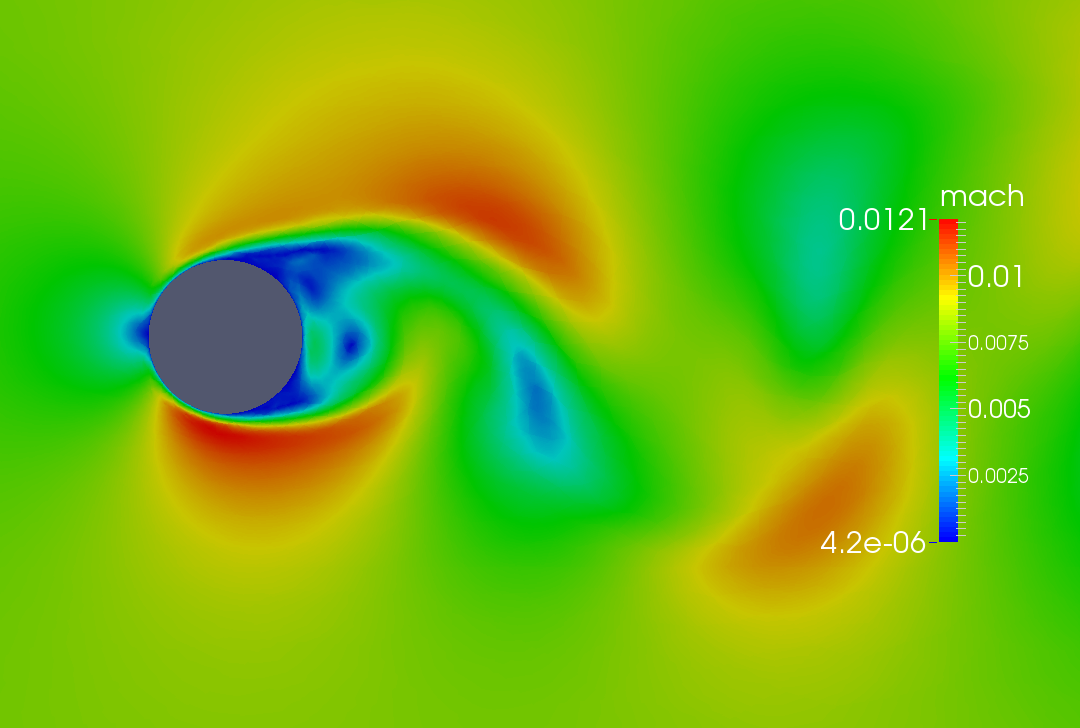
\includegraphics[width=0.55\textwidth]{\lfsdir/figs/Ma0_0077--Re1e6_Ma_closeup.png}
}
\caption{Flow past a cylinder. \gls{re}$= 1e6$, \gls{ma} $= 0.0077, p = 4$}
\label{fig:Ma0.0077Re1e6_Ma}

\end{figure*}

% !TEX root = ./thesis.tex
\subsection{Effects of Filtering in a Well-resolved Simulation}
\label{sec:filteringEffects}

This Section shows that the use of \gls{lfs} has effects similar to using artificial viscosity. The previous results show that \gls{lfs} filters can stabilize even the most extreme of circumstances. What about the effect of using \gls{lfs} filters in more reasonable conditions?

The case of 2-D flow over a circular cylinder at \gls{re} $=3,900$, \gls{ma} $=0.1$ has been selected given the good amount of computational results for it. The thesis by Beaudan \cite{beaudan1994numerical} provides a very thorough discussion of the physics of the 3-D problem and results of simulations with structured high-order methods.

At \gls{re} $=3,900$, a proper simulation of flow around a circular cylinder must be 3-D \cite{breuer1998large}. In fact, previous 2-D simulations of this case have shown the flow to be highly asymmetric \cite{breuer1998large}. The aim of the simulations presented here is not to predict experimental results, but rather to provide an understanding of how the flow will be affected by the use of \gls{lfs} filters. We will see that the \gls{lfs} filters act as artificial viscosity: flow that would otherwise exhibit chaotic behavior becomes periodic. A similar transition from chaotic to periodic behavior due to added dissipation (via turbulence modeling) has been observed in \gls{urans} simulations \cite{catalano2003numerical}.

\subsubsection{Setup}
\label{sec:filterEffectsSetup}

We first generate a grid for a $2^{\mathrm{nd}}$ order method that resolves the $y+$ scales around the cylinder. We then generate grids that maintain close to the same number of \gls{dof} for a \nth{5}  and \nth{6} spatial order of accuracy scheme. We perform the simulation of \gls{re}$=3.9e3$ past a circular cylinder using the \nth{5} and \nth{6} order schemes in the different grids. The aims of this setup are to:
\begin{enumerate}
\item Have a well-resolved, baseline case
\item Visualize the effects of changing the spatial order of accuracy while maintaining the number of \gls{dof} almost constant
\item Visualize the effects of using an under-resolved grid
\item Visualize the effects of using \gls{lfs} filters in different grids with different spatial orders of accuracy
\end{enumerate}

A baseline case with a \nth{6} order accurate in space scheme was attempted while maintaining the same number of degrees of freedom as the case with the $2^{\mathrm{nd}}$ order scheme. However, the non-linearities within the relatively large elements elements prevented the simulation from completing without intervention. However, a simulation with filtering in the same grid with the same order of accuracy did run to completion.

In addition, to compare the effects of filtering versus running a slightly unresolved simulation, an unfiltered case of a slightly unresolved grid was run with a \nth{5} order scheme.

Finally, a well resolved, yet filtered, simulation with the \nth{5} order scheme was performed.

All cases ran with the same non-dimensional time-step of $\Delta t = 1e-5$ for a non-dimensional time of $t = 64.7$. Given that \gls{ma} $=0.1$, temperature of air simulated was $300K$, $\gamma = 1.4$, and the reference length was $1$ meter, the physical time-step was $2.88e-6$ seconds and the physical simulation time was $1.86$ seconds.

Filtering is performed with a value of $h = 10$ in Equation \eqref{eq:sharp_spectral} and $\alpha = 0.8$ in Equation \eqref{eqn:filter_form}. All conservation fields are filtered every 500 time-steps, so every $5e-2$ non-dimensional time units, or every $1.44e-3$ seconds. The filtering procedure was kept the same to isolate the effects of filtering. In practice, a sensor should be used in order to only filter the elements where instabilities could arise.


\subsubsection{Results and Discussion}
\label{sec:filterEffectsResults}

Table \ref{table:filteringEffect_simSummary} summarizes all the cases run and provides hyperlinks to videos of the resulting flow simulations. The value of \gls{st} provided reflects the peak \gls{st} of the lift coefficient power spectrum.

All cases display the following phases: a pair of vortices strengthen behind the cylinder, the vortices elongate and the drag coefficient decreases, asymmetries in the solution trigger vortex shedding, the vortex growth and shedding process transitions into a quasiperiodic (when not filtered) or periodic (when filtered) behavior.

\begin{table}
%\begin{adjustwidth}{-2.1cm}{}
%    \centering
\cellspacebottomlimit=5pt
\cellspacetoplimit=5pt
%      \begin{center}                % keep track of old \tabcolsep
\setlength{\oldtabcolsep}{\tabcolsep}     % 6.0pt
\setlength{\tabcolsep}{0pt}               % so coloring doesn't run off
% ends of the table
\renewcommand{\arraystretch}{2}         % because math expressions
% almost run into each other

\def \spacing {0.4cm}
\hspace{-0.5cm}
\begin{tabular}{c <{\hspace{\len}} c <{\hspace{\len}} c <{\hspace{\len}} c <{\hspace{\spacing}} 
c <{\hspace{\spacing}}
c<{\hspace{\spacing}} c<{\hspace{\spacing}} c<{\hspace{\spacing}} c}
\toprule
Case & $P$  & Mesh & Filtered & Grid & $\#$ \gls{dof} & \specialcell[b]{$C_L$ and $C_D$ vs. $t$ \vspace{-0.2cm}\\Figure}   &  \specialcell[b]{\gls{st}} & \specialcell[b]{Video} \\
\specialrule{\lightrulewidth}{0pt}{0pt} % so row-coloring aligns

\hypertarget{caseA}{A} & 1 &  \ref{fig:mesh_case_A} & No & \ref{fig:mesh_case_A} & 1,579,620 & \ref{fig:history_P1_noFilt_mesh1} & 0.19 & \href{https://www.youtube.com/watch?v=mtUrv-Aj_y0}{link} \\
\hypertarget{caseB}{B} & 4 & \ref{fig:mesh_case_BDG} & No & \ref{fig:mesh_case_BDG} & 1,398,780 & \ref{fig:history_P4_noFilt_mesh4} & 0.17 & \href{https://www.youtube.com/watch?v=FpyAf08kz7A}{link} \\
\hypertarget{caseC}{C} & 4 & \ref{fig:mesh_case_C} & No & \ref{fig:mesh_case_C} & 703,260 & \ref{fig:history_P4_noFilt_mesh6} & 0.17 & \href{https://www.youtube.com/watch?v=Tud7N1tmmrA}{link} \\
\hypertarget{caseD}{D} & 4 & \ref{fig:mesh_case_BDG} & Yes & \ref{fig:mesh_case_BDG} & 1,398,780 & \ref{fig:history_P4_filt_mesh4} & 0.25 & \href{https://youtu.be/H1xKenZ2g6Q}{link} \\
\hypertarget{caseE}{E} & 5 & \ref{fig:mesh_case_EF} & No & \ref{fig:mesh_case_EF} & 1,362,396 & Unstable & N/A & N/A \\
\hypertarget{caseF}{F} & 5 & \ref{fig:mesh_case_EF} & Yes & \ref{fig:mesh_case_EF} & 1,362,396 & \ref{fig:history_P5_filt_mesh5} & 0.21 & \href{https://www.youtube.com/watch?v=FMZBi285alk}{link} \\
\hypertarget{caseG}{G} & 5 & \ref{fig:mesh_case_BDG} & Yes & \ref{fig:mesh_case_BDG} & 1,958,292 & \ref{fig:history_P5_filt_mesh4} & 0.25 & \href{https://www.youtube.com/watch?v=cmIKRwJXoME}{link} \\

\bottomrule
\end{tabular}
\caption{Simulation results that illustrate effect of filtering, changing meshes, and varying the spatial order of accuracy. All cases were run at \gls{ma} $=0.1$, \gls{re}$ = 3.9e3$.}
\label{table:filteringEffect_simSummary}
\end{table}


\begin{figure}
\centering
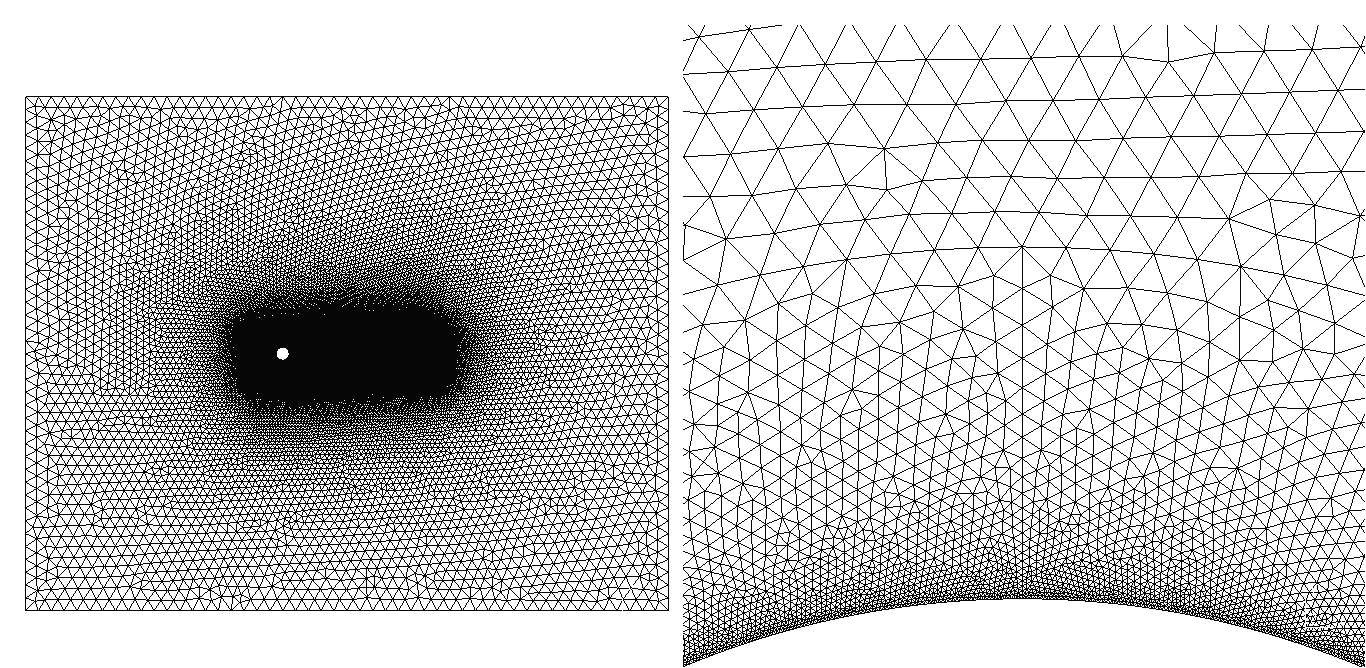
\includegraphics[width = 1\textwidth]{\lfsdir/figs/mesh_images/cylinder_1stOrder_Re3-6e3_fine1_mod.png}
\caption{Mesh used in case A in Table \ref{table:filteringEffect_simSummary}. Contains 131,635 triangular elements with second order edges.} 
\label{fig:mesh_case_A}
\end{figure}

\begin{figure}
\centering
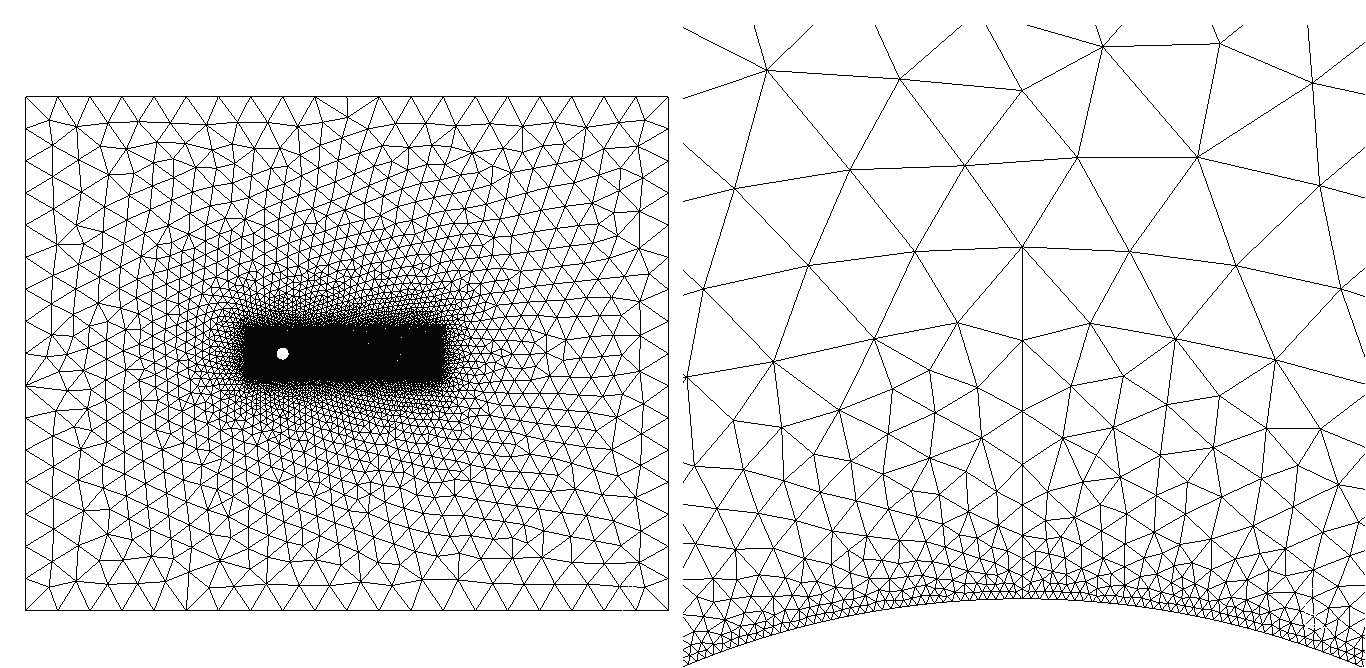
\includegraphics[width = 1\textwidth]{\lfsdir/figs/mesh_images/cylinder_4thOrder_Re3-9e3_mod.png}
\caption{Mesh used in cases B, D, and G in Table \ref{table:filteringEffect_simSummary}. Contains 23,313 triangular elements with second order edges.} 
\label{fig:mesh_case_BDG}
\end{figure}

\begin{figure}
\centering
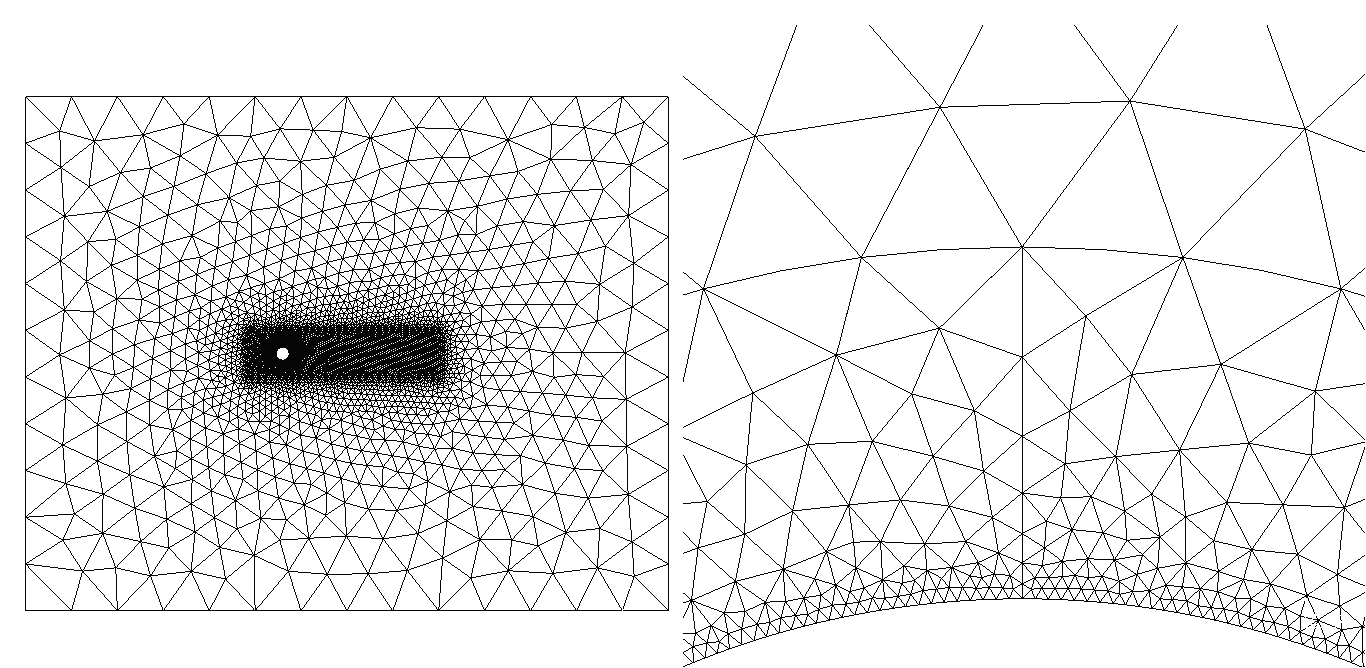
\includegraphics[width = 1\textwidth]{\lfsdir/figs/mesh_images/cylinder_6thOrder_Re3-9e3_mod.png}
\caption{Mesh used in case C in Table \ref{table:filteringEffect_simSummary}. Contains 11,721 triangular elements with second order edges.} 
\label{fig:mesh_case_C}
\end{figure}

\begin{figure}
\centering
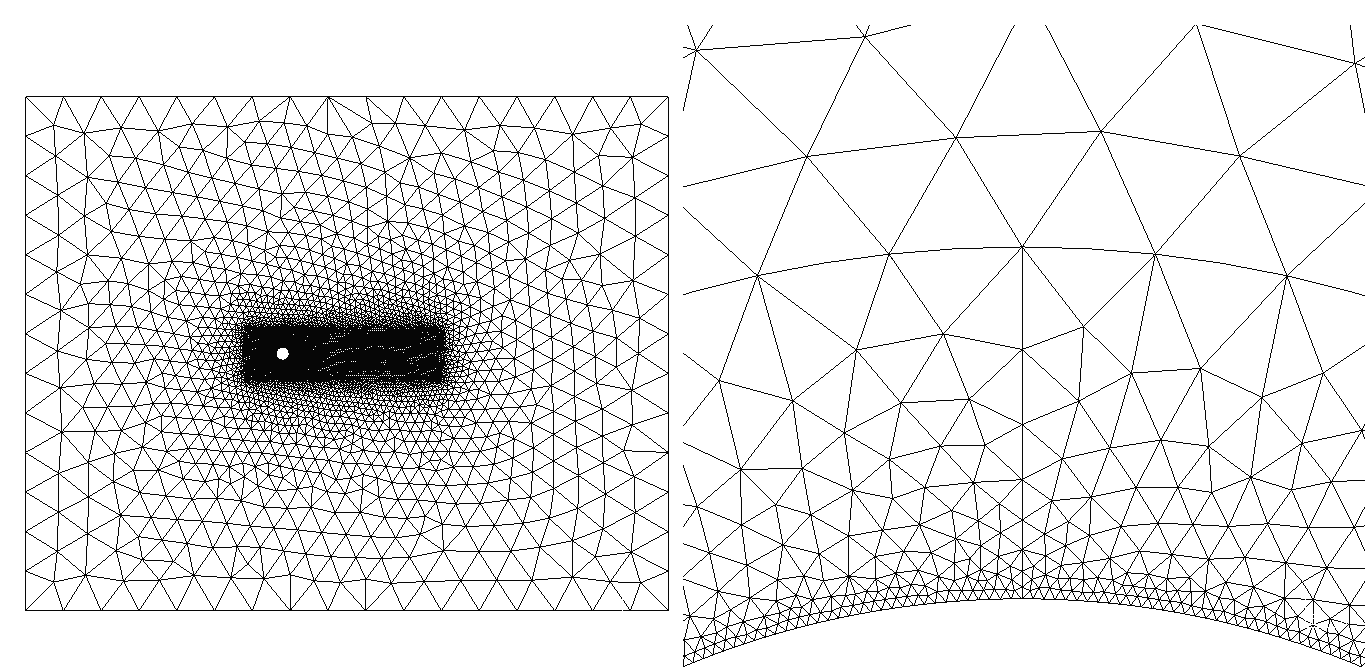
\includegraphics[width = 1\textwidth]{\lfsdir/figs/mesh_images/cylinder_5thOrder_Re3-9e3_mod.png}
\caption{Mesh used in cases E and F in Table \ref{table:filteringEffect_simSummary}. Contains 16,219 triangular elements with second order edges.}
\label{fig:mesh_case_EF}
\end{figure}

% % % % % % % % % % % % % % % % % % % % % % % %  Simulation Results

\begin{figure}
\centering
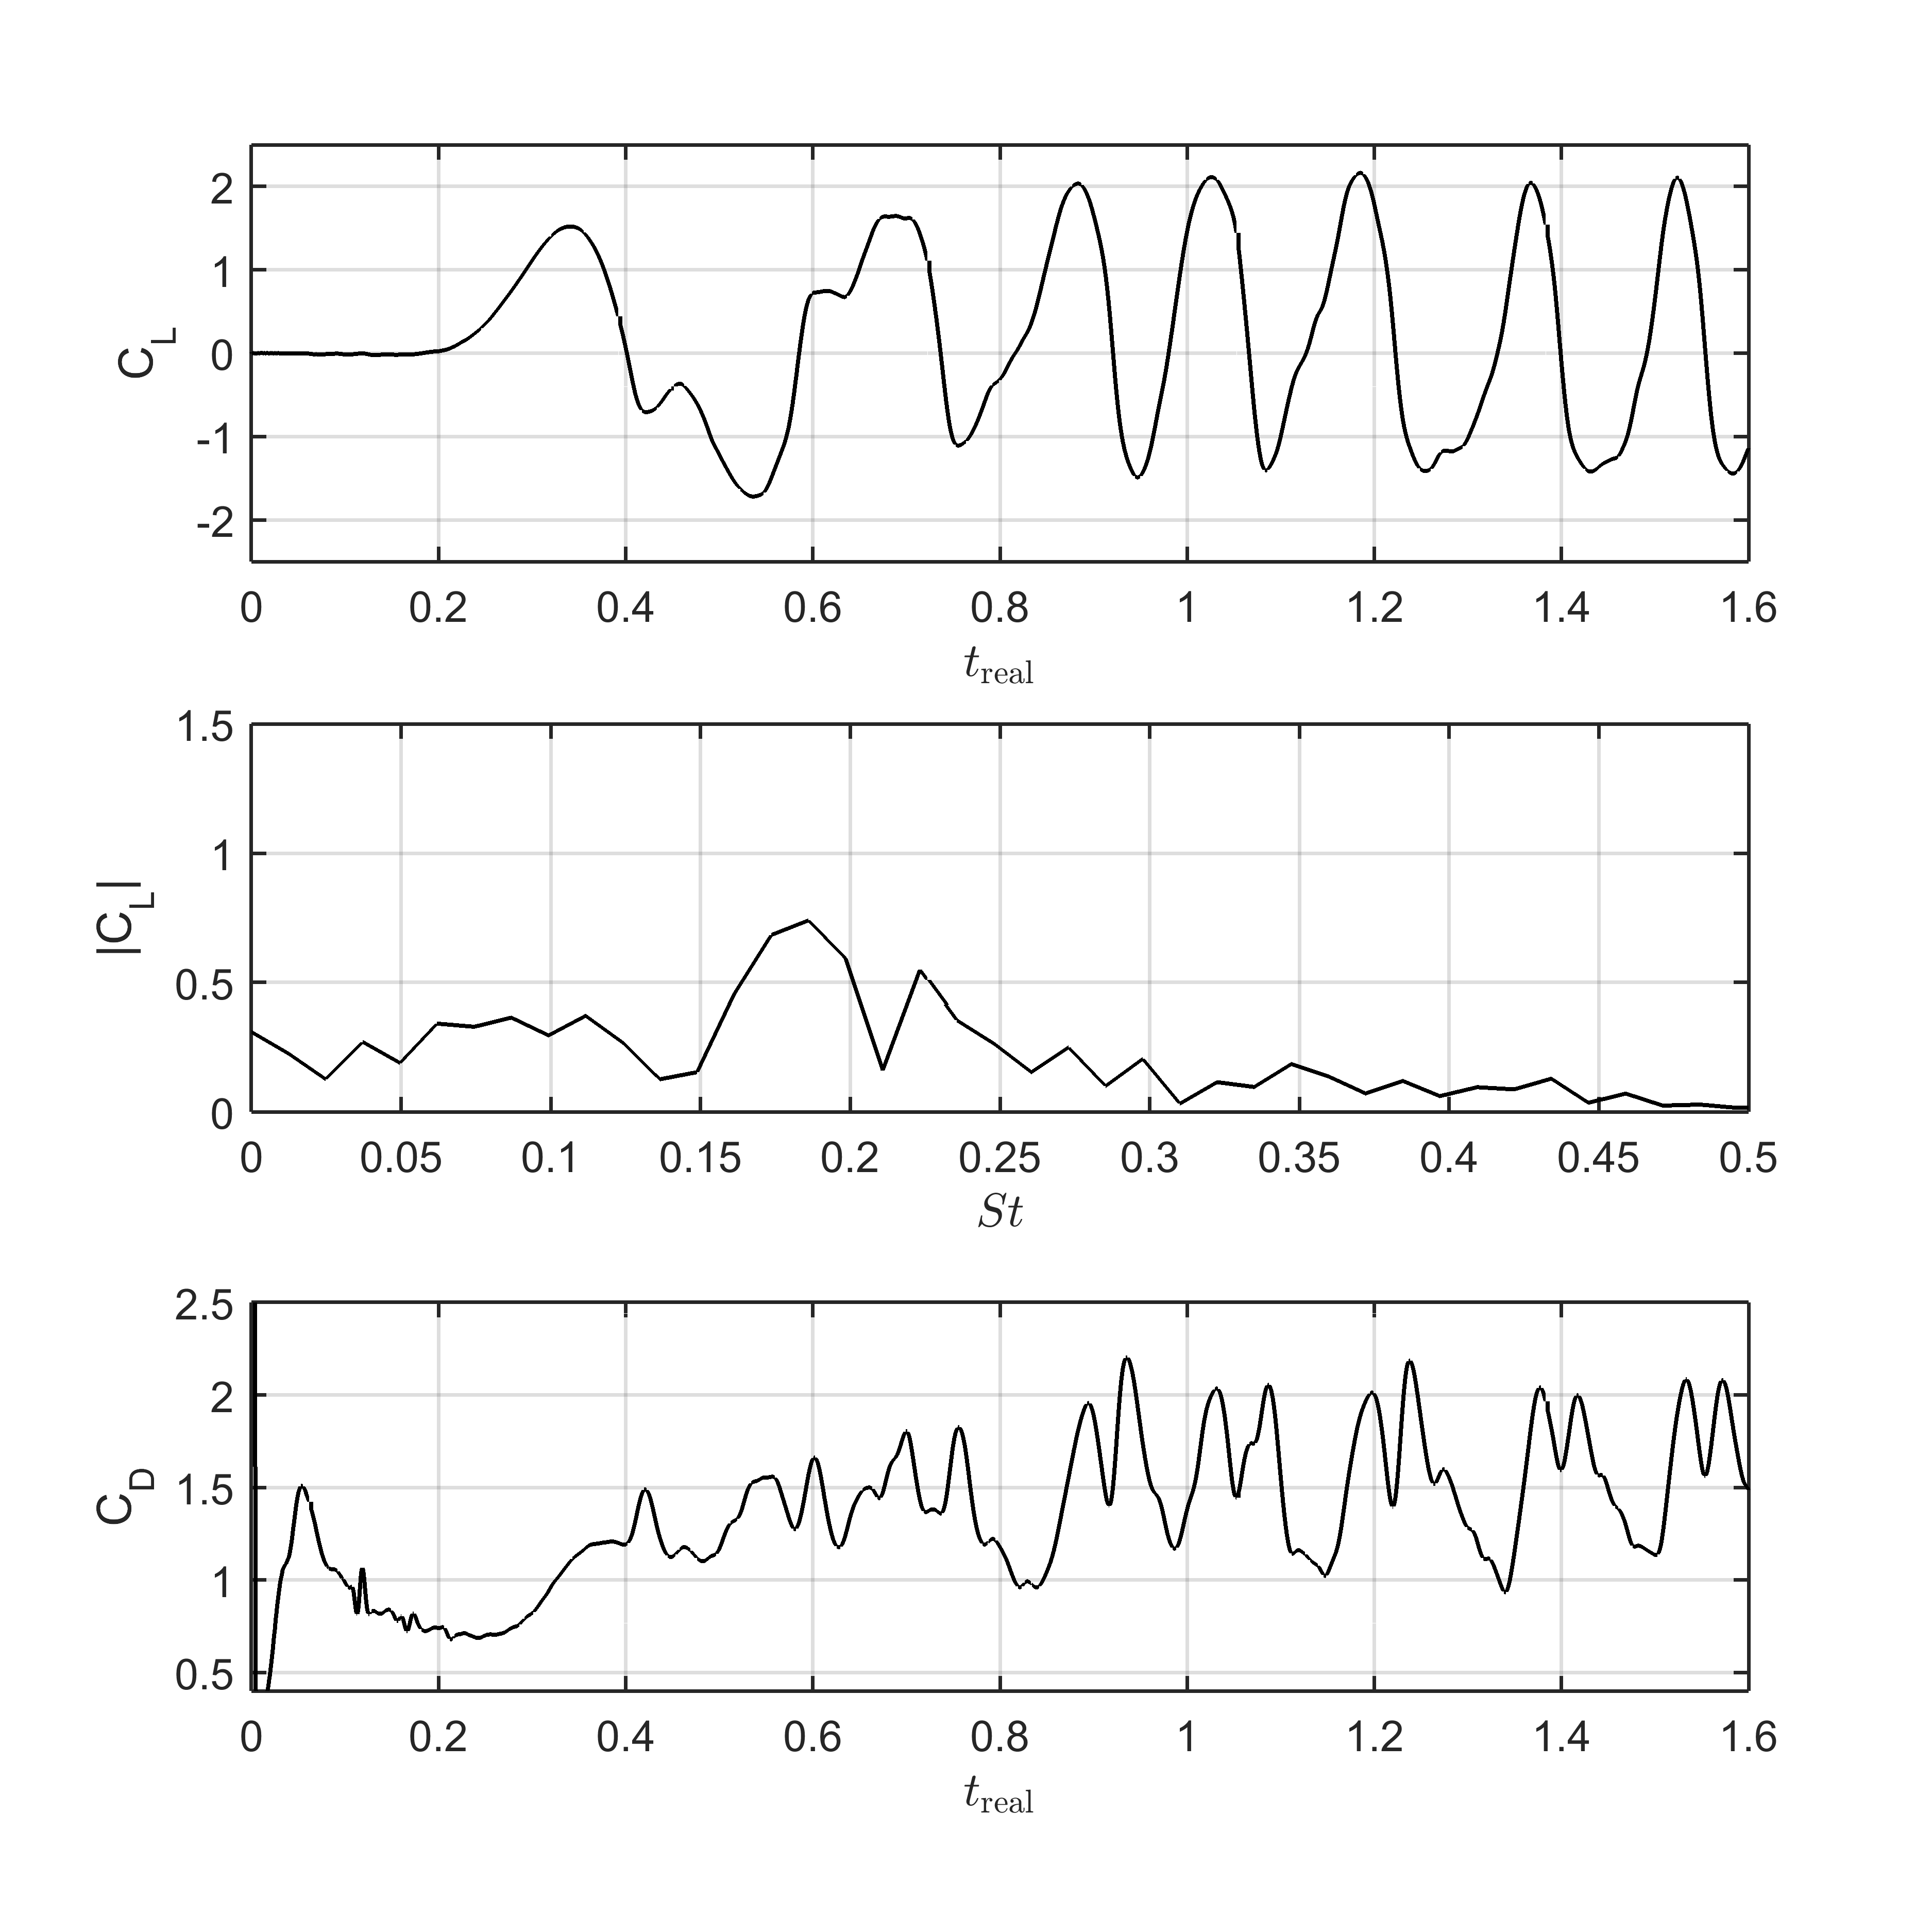
\includegraphics[width = 1\textwidth]{\lfsdir/figs/history_P1_noFilt_mesh1.png}
\caption{Case A in Table \ref{table:filteringEffect_simSummary} lift coefficient, \gls{st} power spectrum, and drag coefficient. Case is not filtered and uses mesh \ref{fig:mesh_case_A} with $P=1$. }  
\label{fig:history_P1_noFilt_mesh1}
\end{figure}

\begin{figure}
\centering
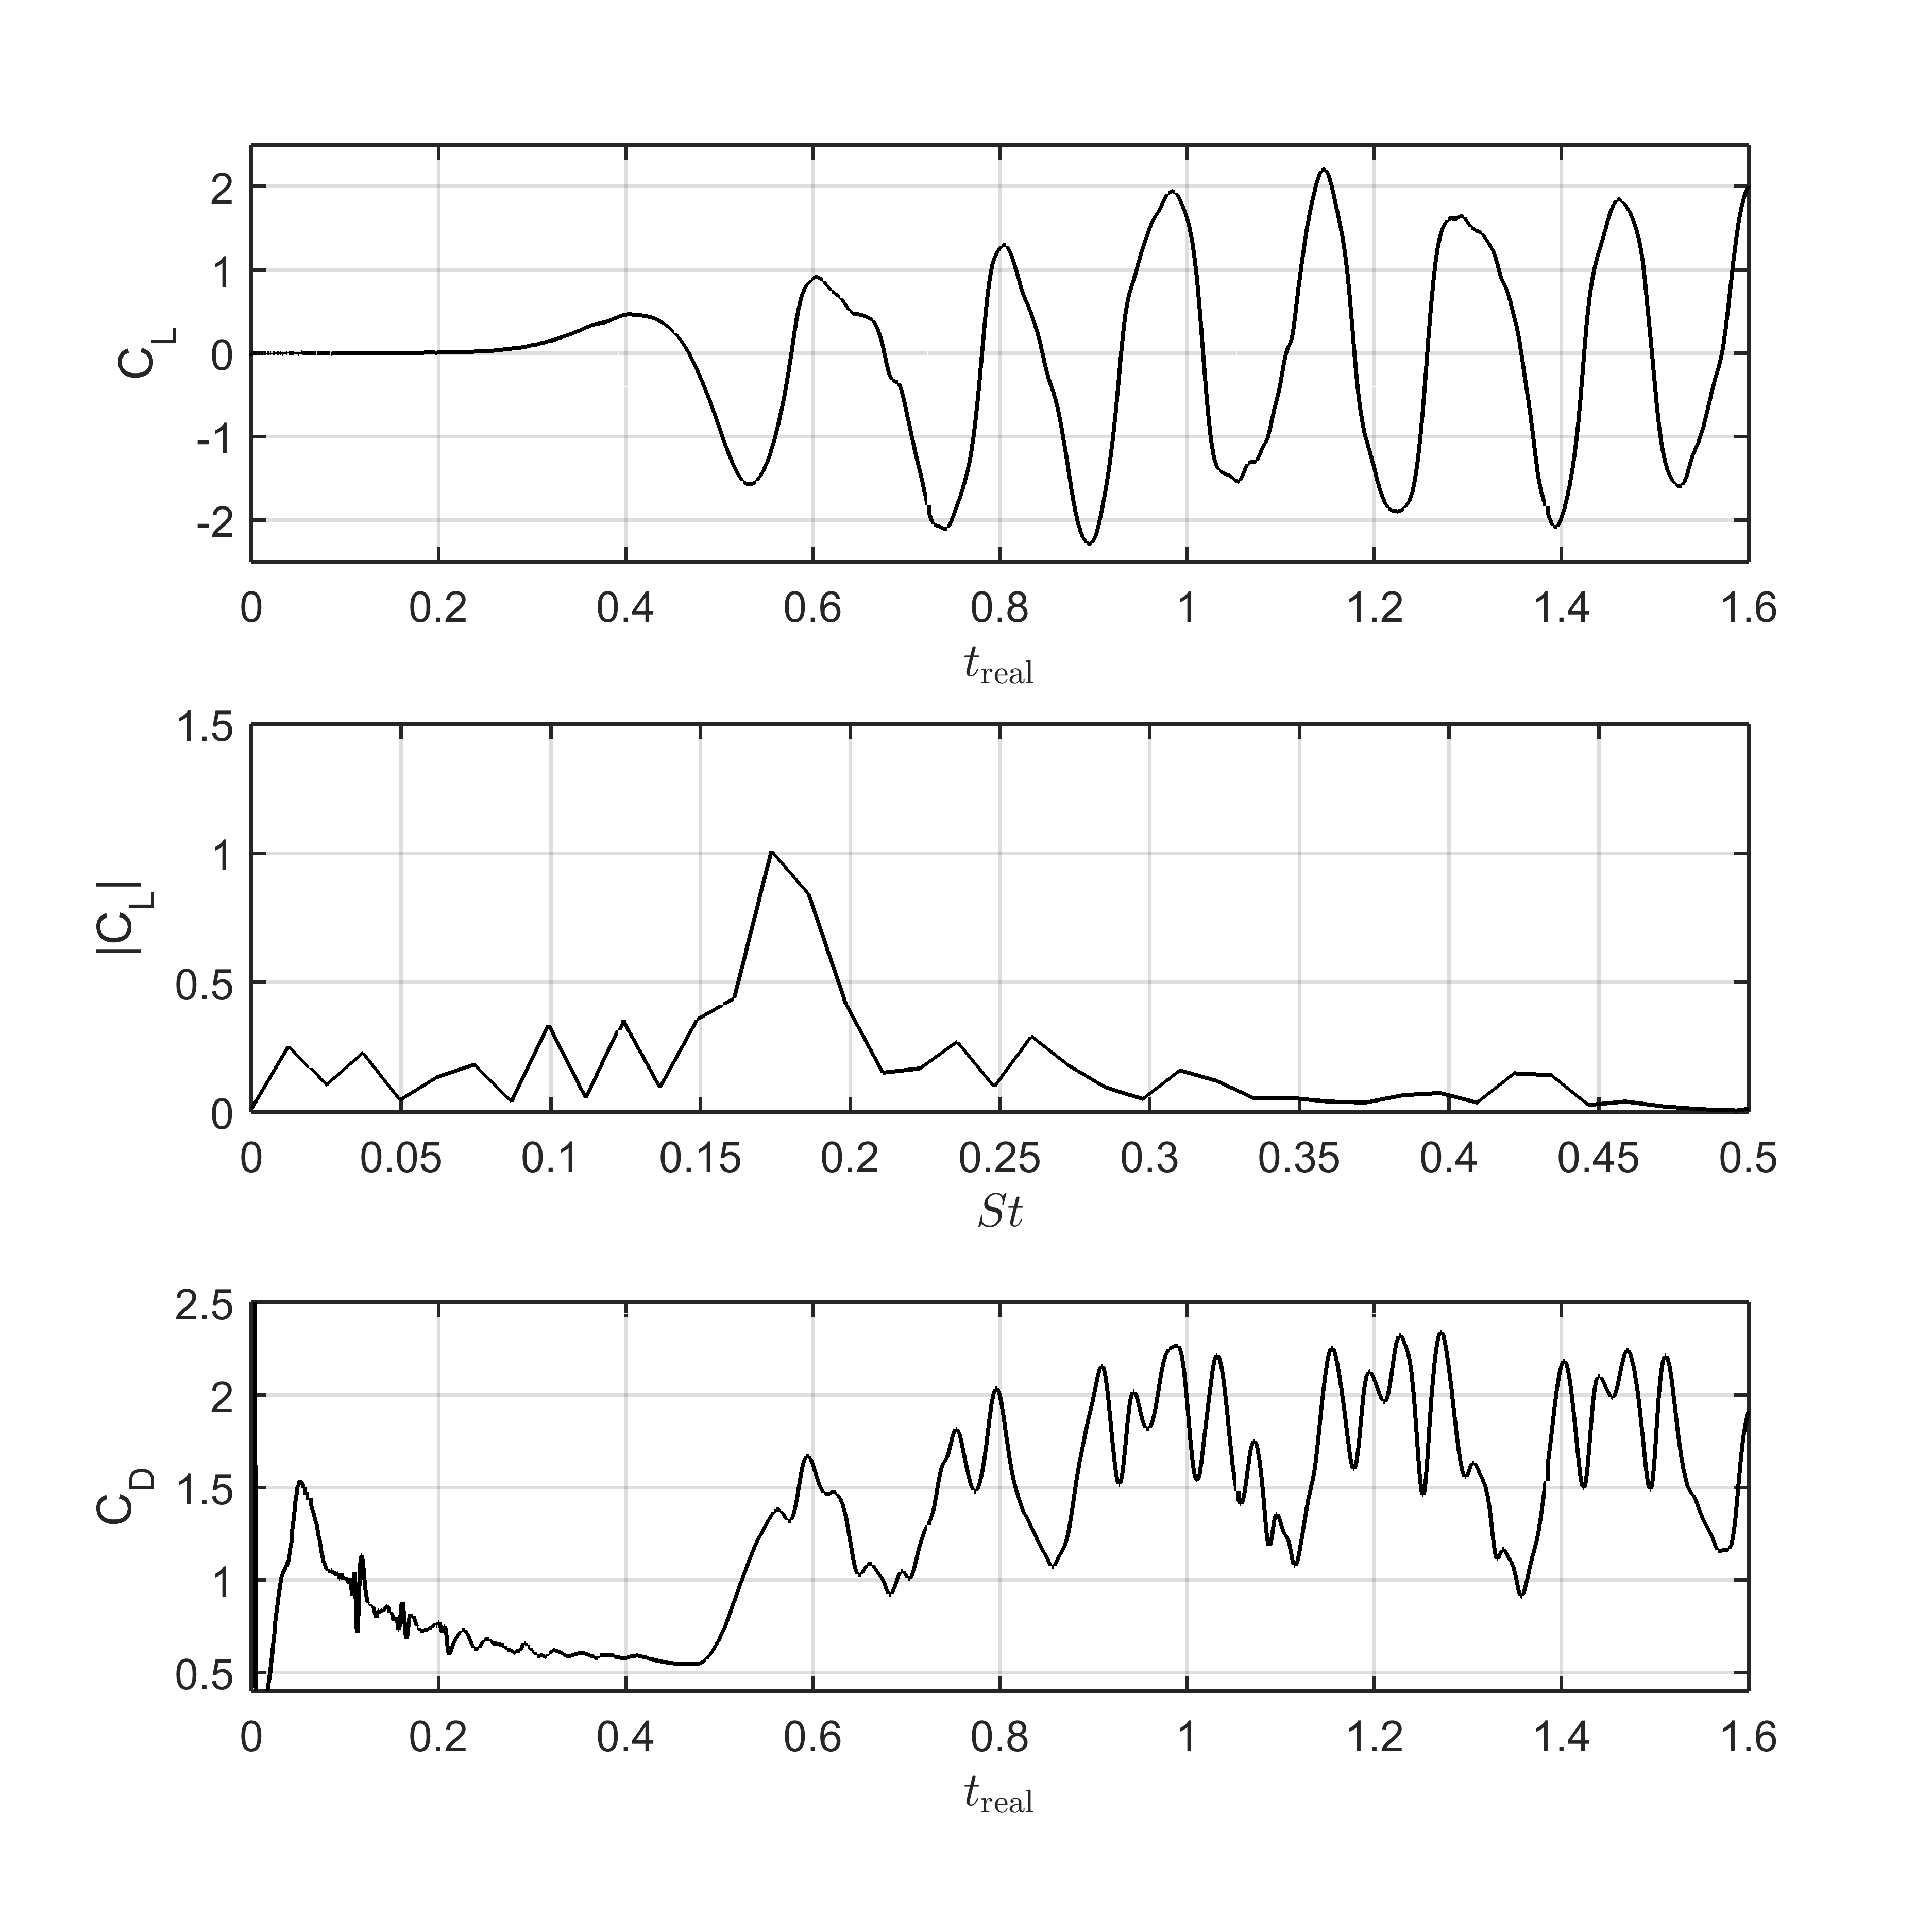
\includegraphics[width = 1\textwidth]{\lfsdir/figs/history_P4_noFilt_mesh4.png}
\caption{Case B in Table \ref{table:filteringEffect_simSummary} lift coefficient, \gls{st} power spectrum, and drag coefficient. Case is not filtered and uses mesh \ref{fig:mesh_case_BDG} with $P=4$.} 
\label{fig:history_P4_noFilt_mesh4}
\end{figure}

\begin{figure}
\centering
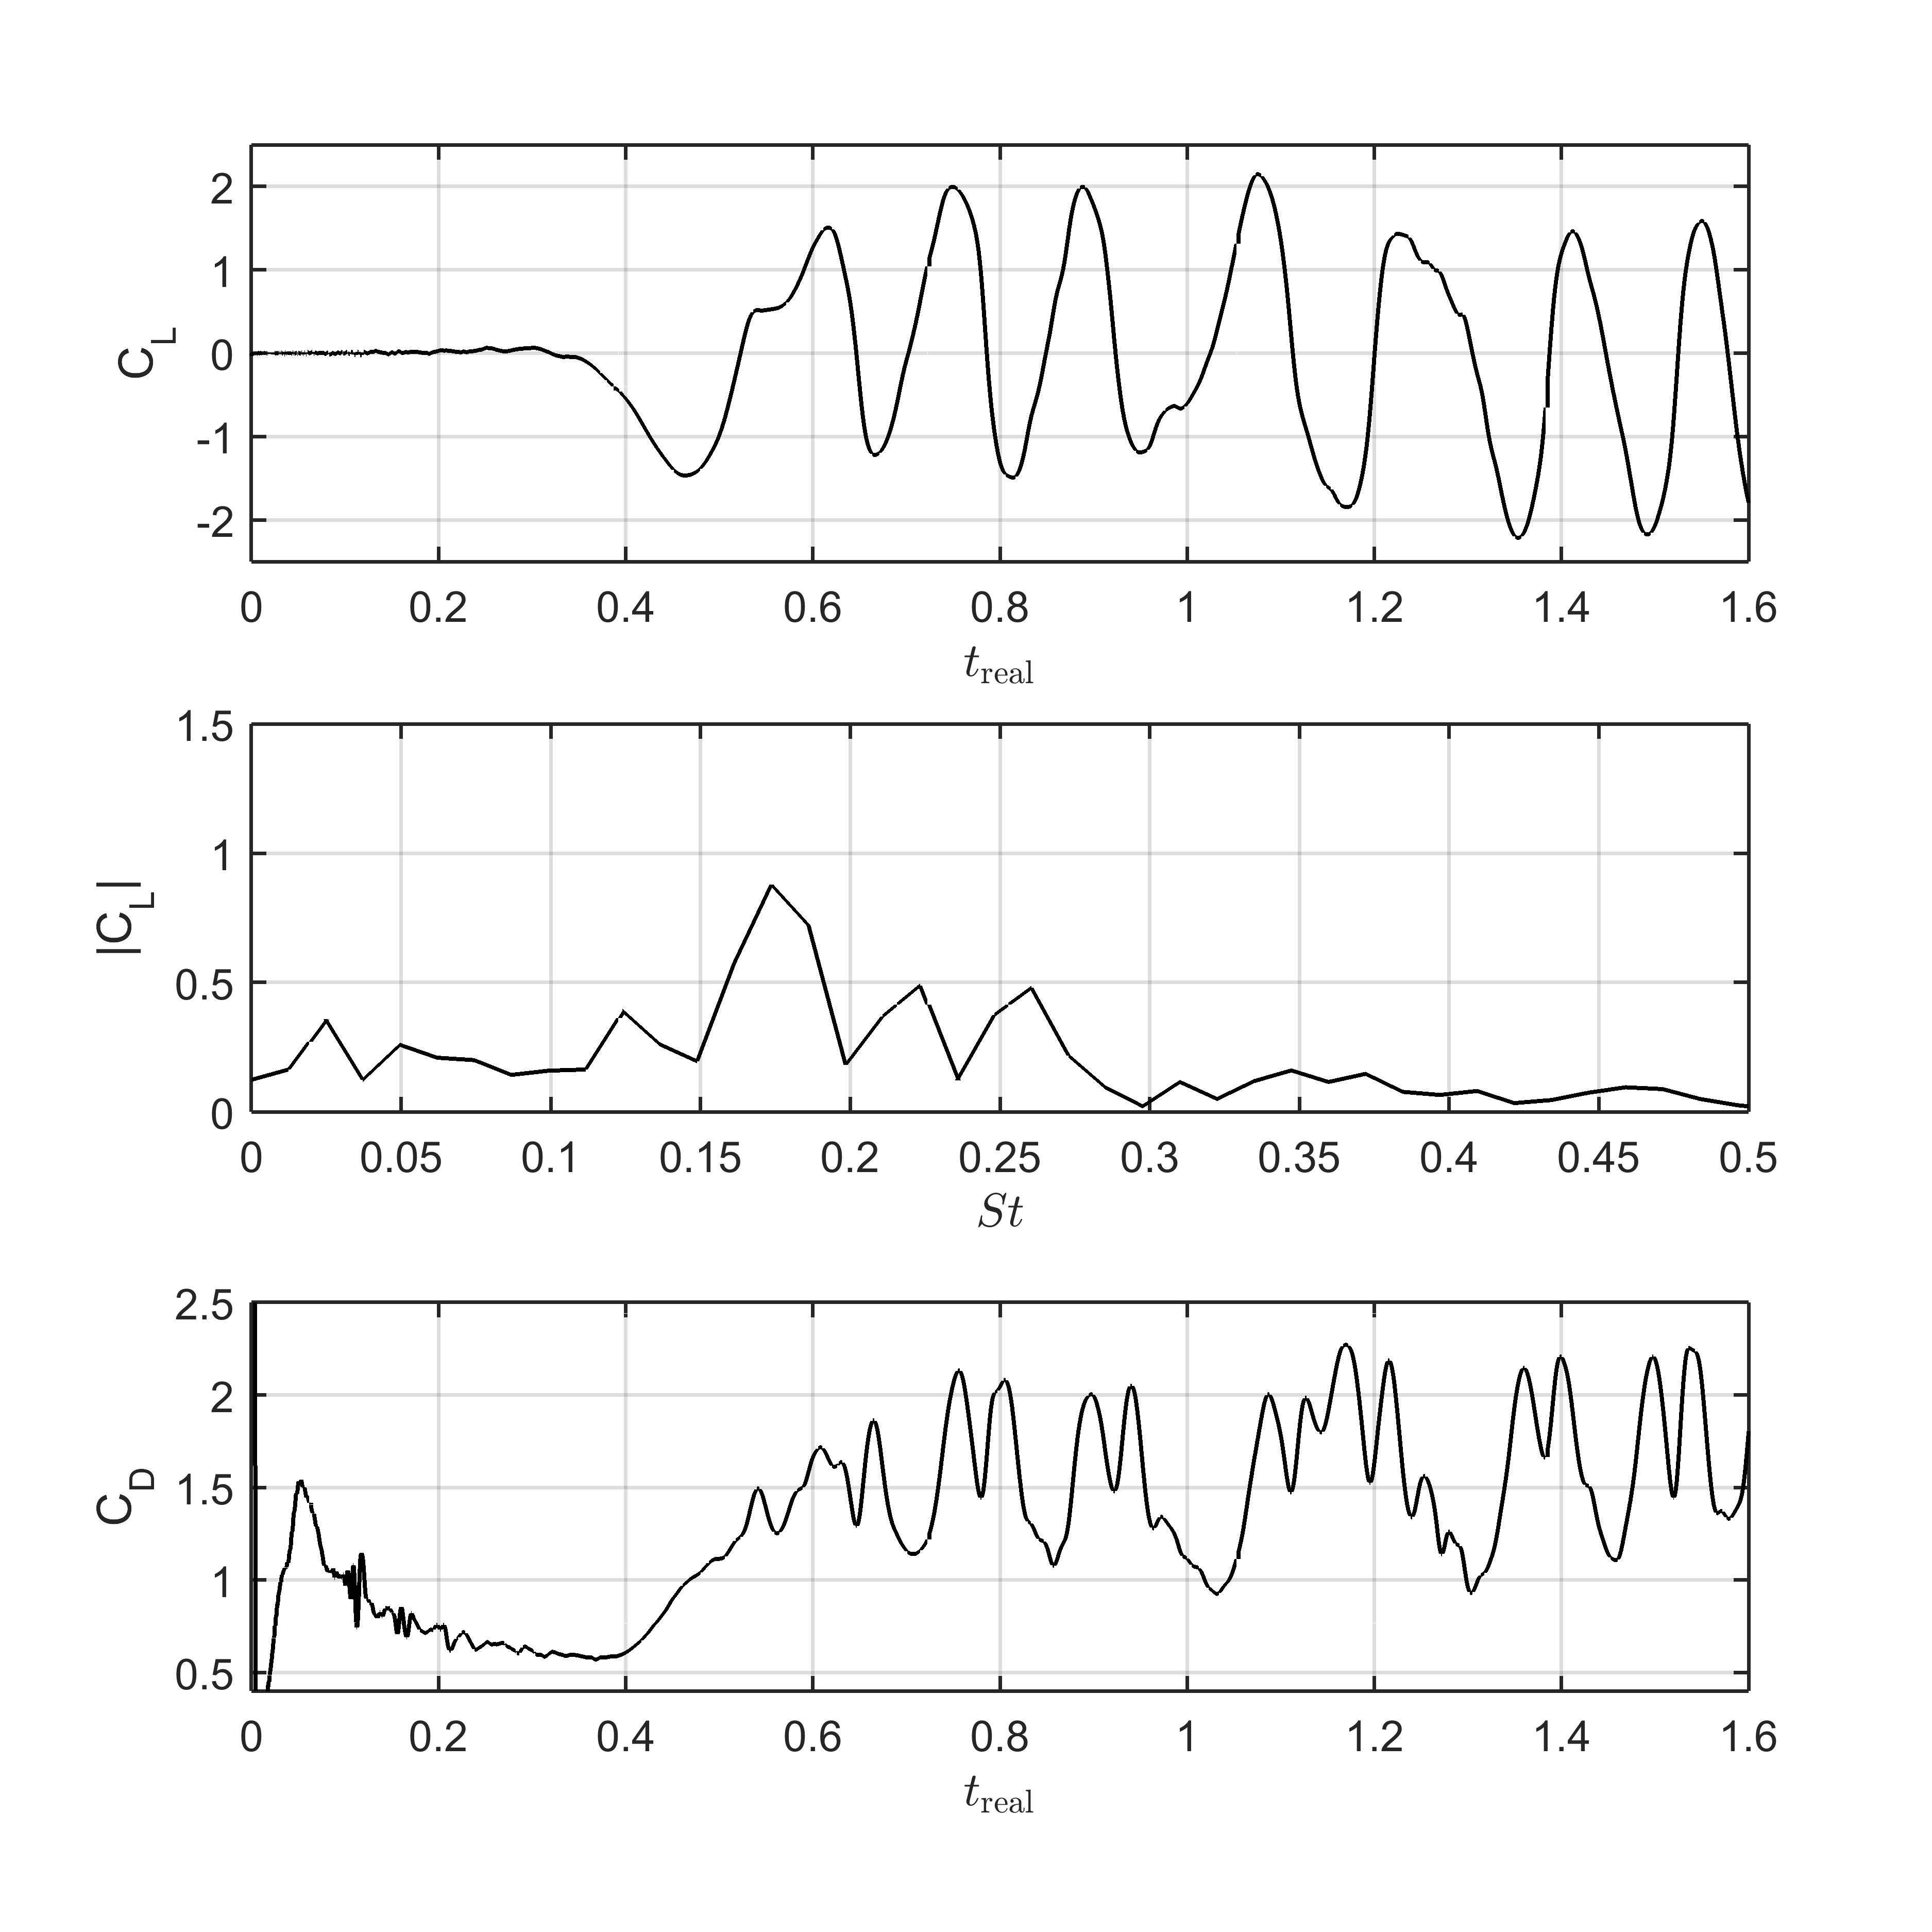
\includegraphics[width = 1\textwidth]{\lfsdir/figs/history_P4_noFilt_mesh6.png}
\caption{Case C in Table \ref{table:filteringEffect_simSummary} lift coefficient, \gls{st} power spectrum, and drag coefficient. Case is not filtered and uses mesh \ref{fig:mesh_case_C} with $P=4$.} 
\label{fig:history_P4_noFilt_mesh6}
\end{figure}

\begin{figure}
\centering
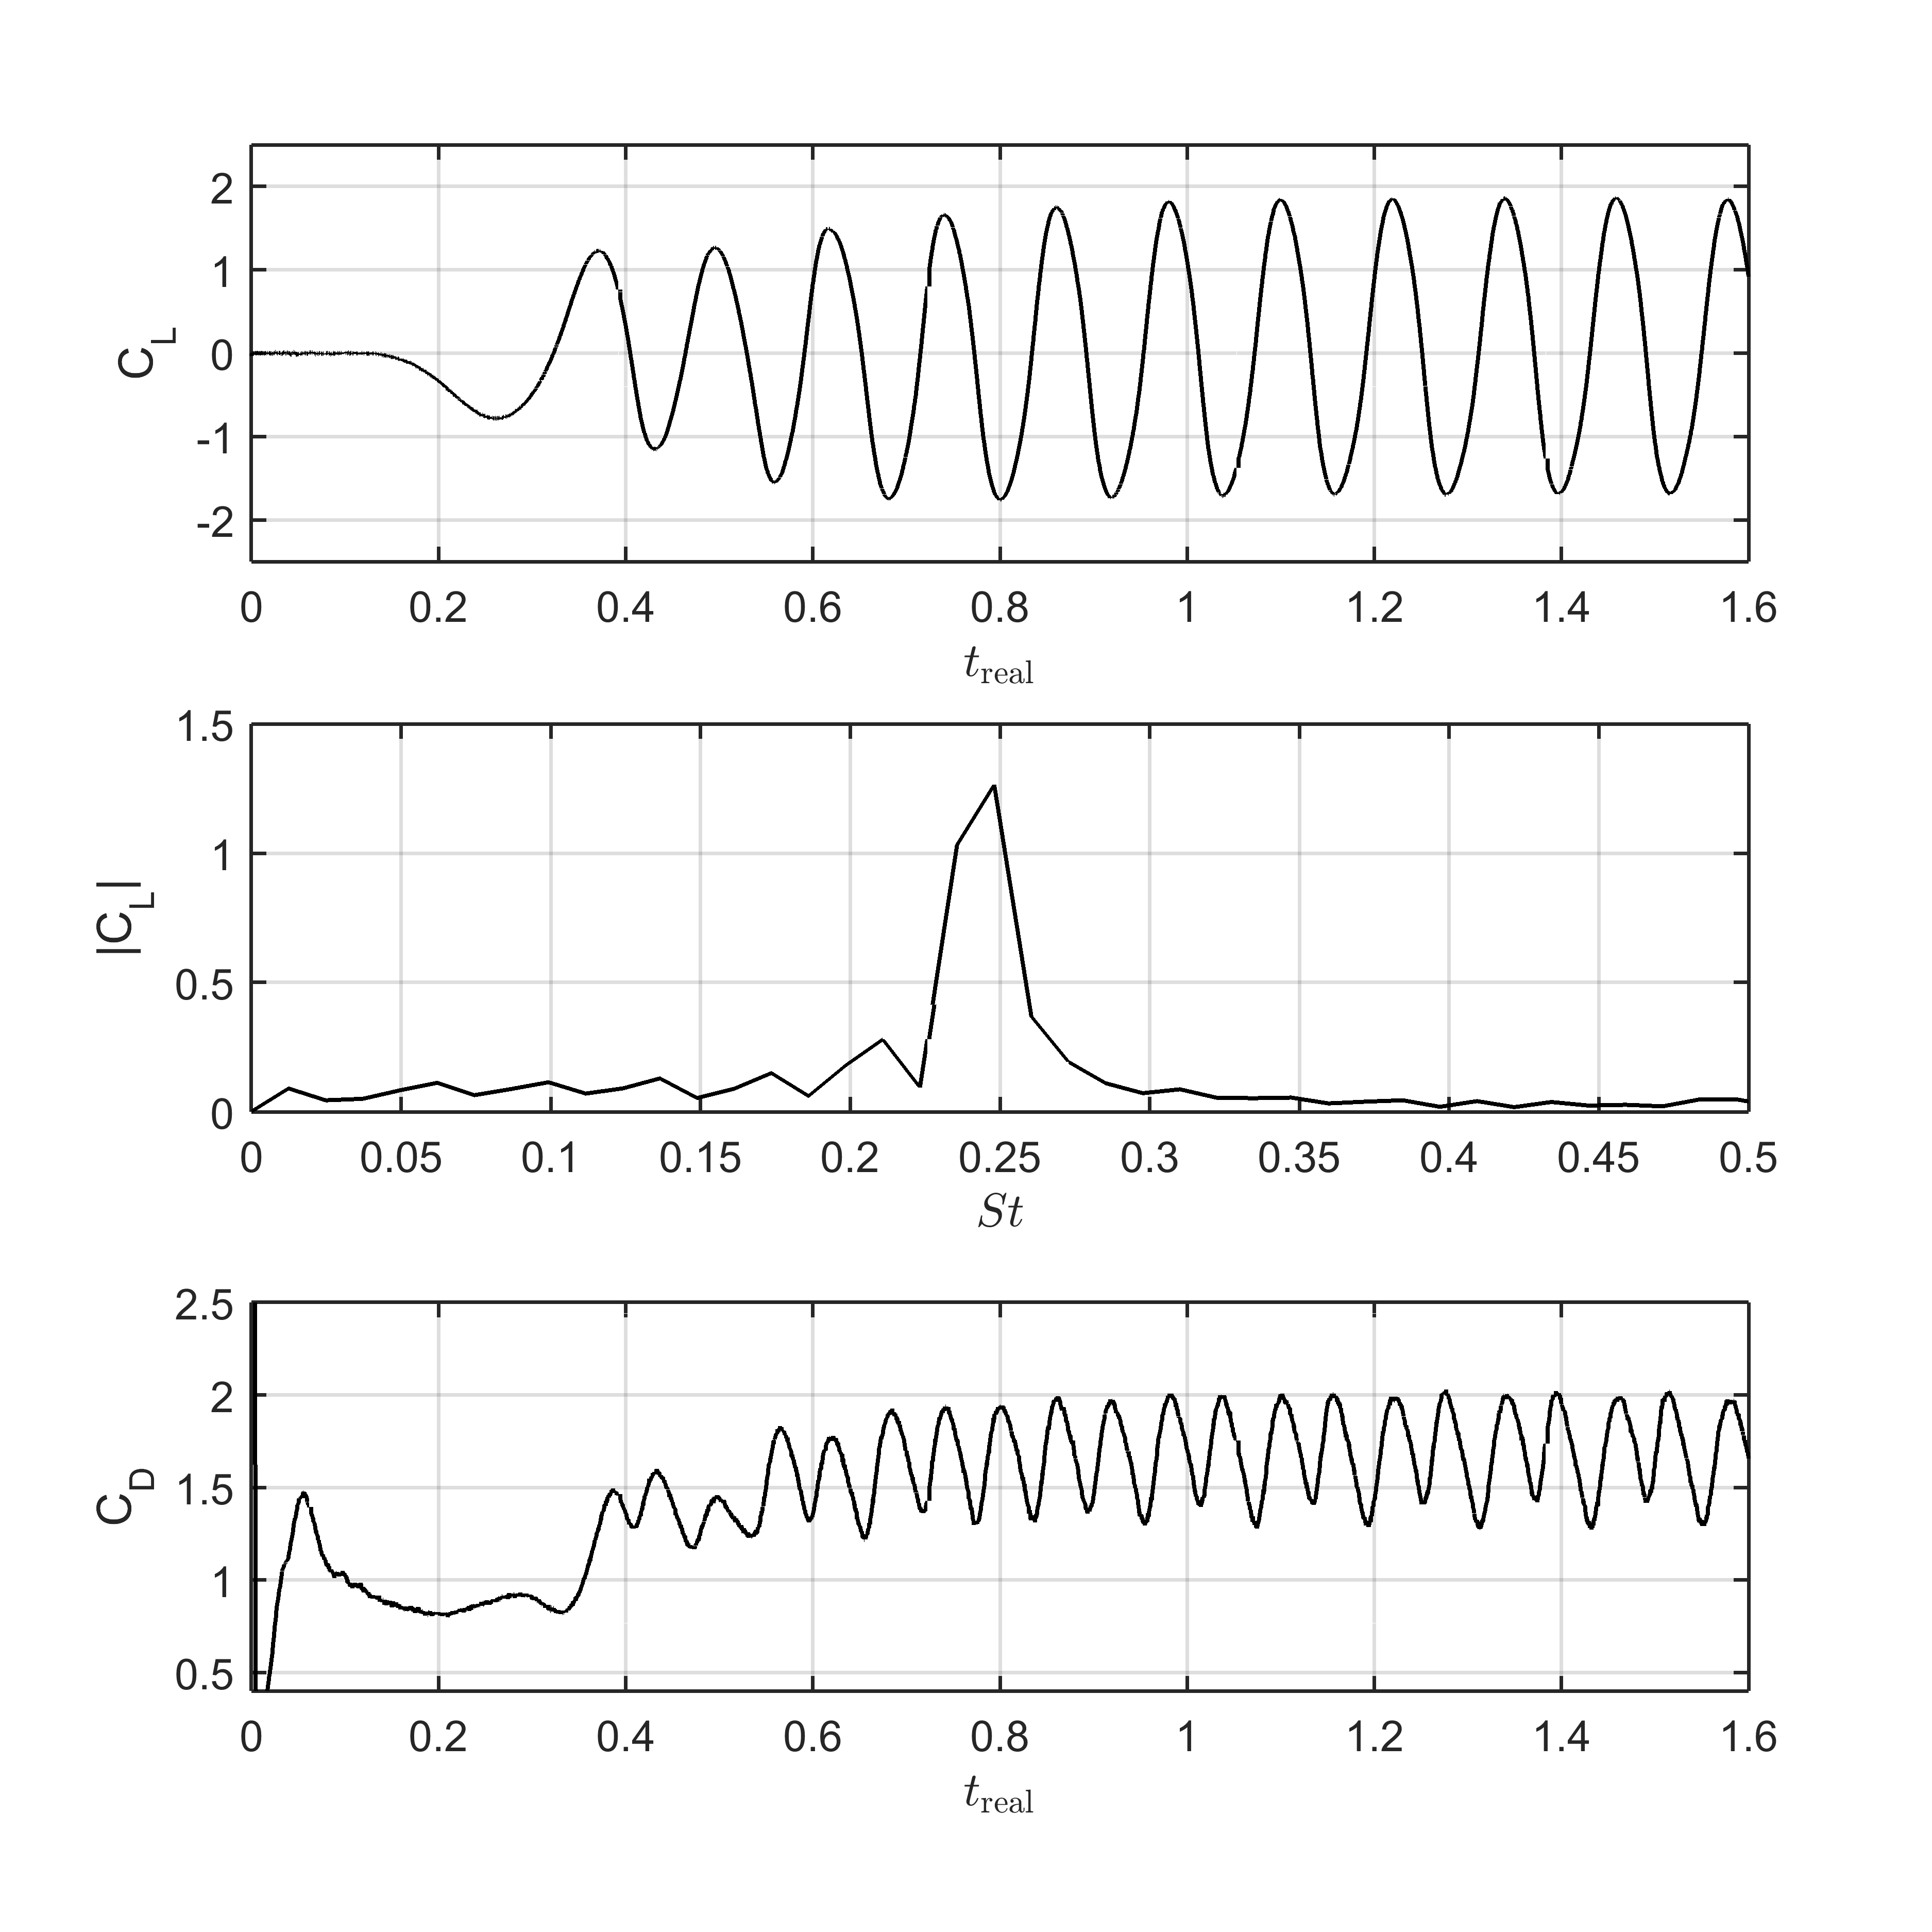
\includegraphics[width = 1\textwidth]{\lfsdir/figs/history_P4_filt_mesh4.png}
\caption{Case D in Table \ref{table:filteringEffect_simSummary} lift coefficient, \gls{st} power spectrum, and drag coefficient. Case is filtered and uses mesh \ref{fig:mesh_case_BDG} with $P=4$.} 
\label{fig:history_P4_filt_mesh4}
\end{figure}

\begin{figure}
\centering
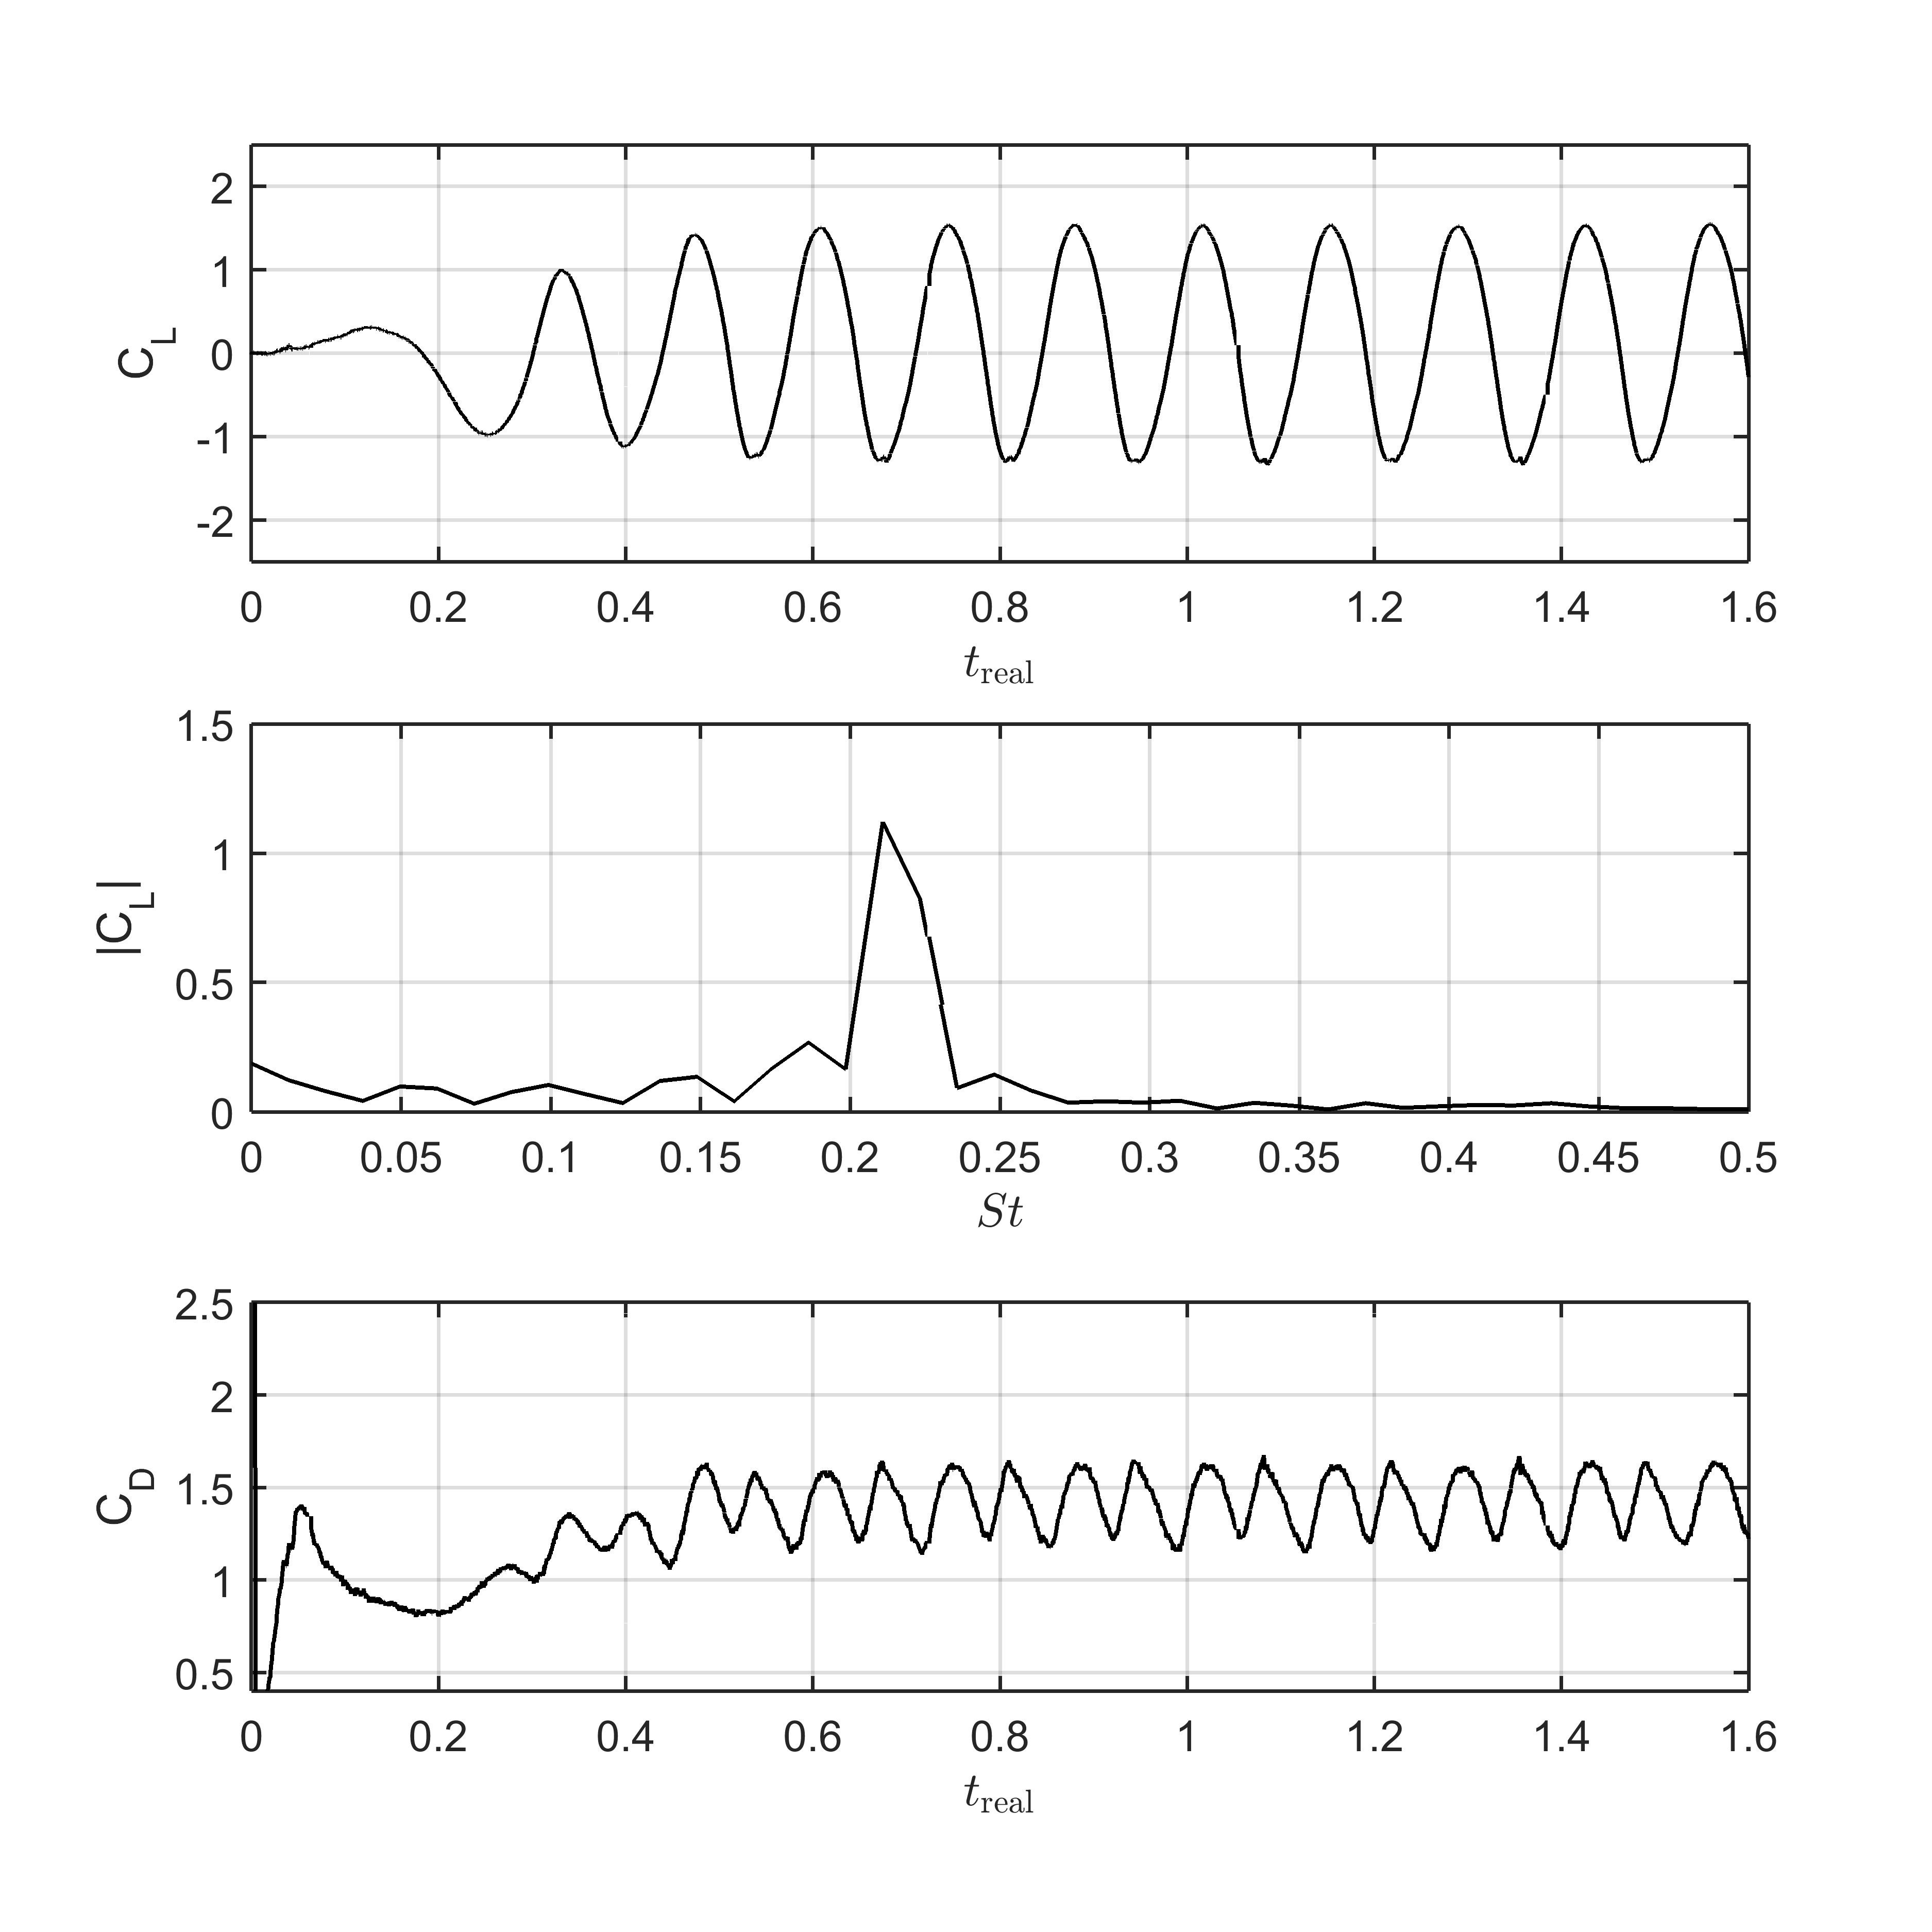
\includegraphics[width = 1\textwidth]{\lfsdir/figs/history_P5_filt_mesh5.png}
\caption{Case F in Table \ref{table:filteringEffect_simSummary} lift coefficient, \gls{st} power spectrum, and drag coefficient. Case is filtered and uses mesh \ref{fig:mesh_case_EF} with $P=5$.} 
\label{fig:history_P5_filt_mesh5}
\end{figure}

\begin{figure}
\centering
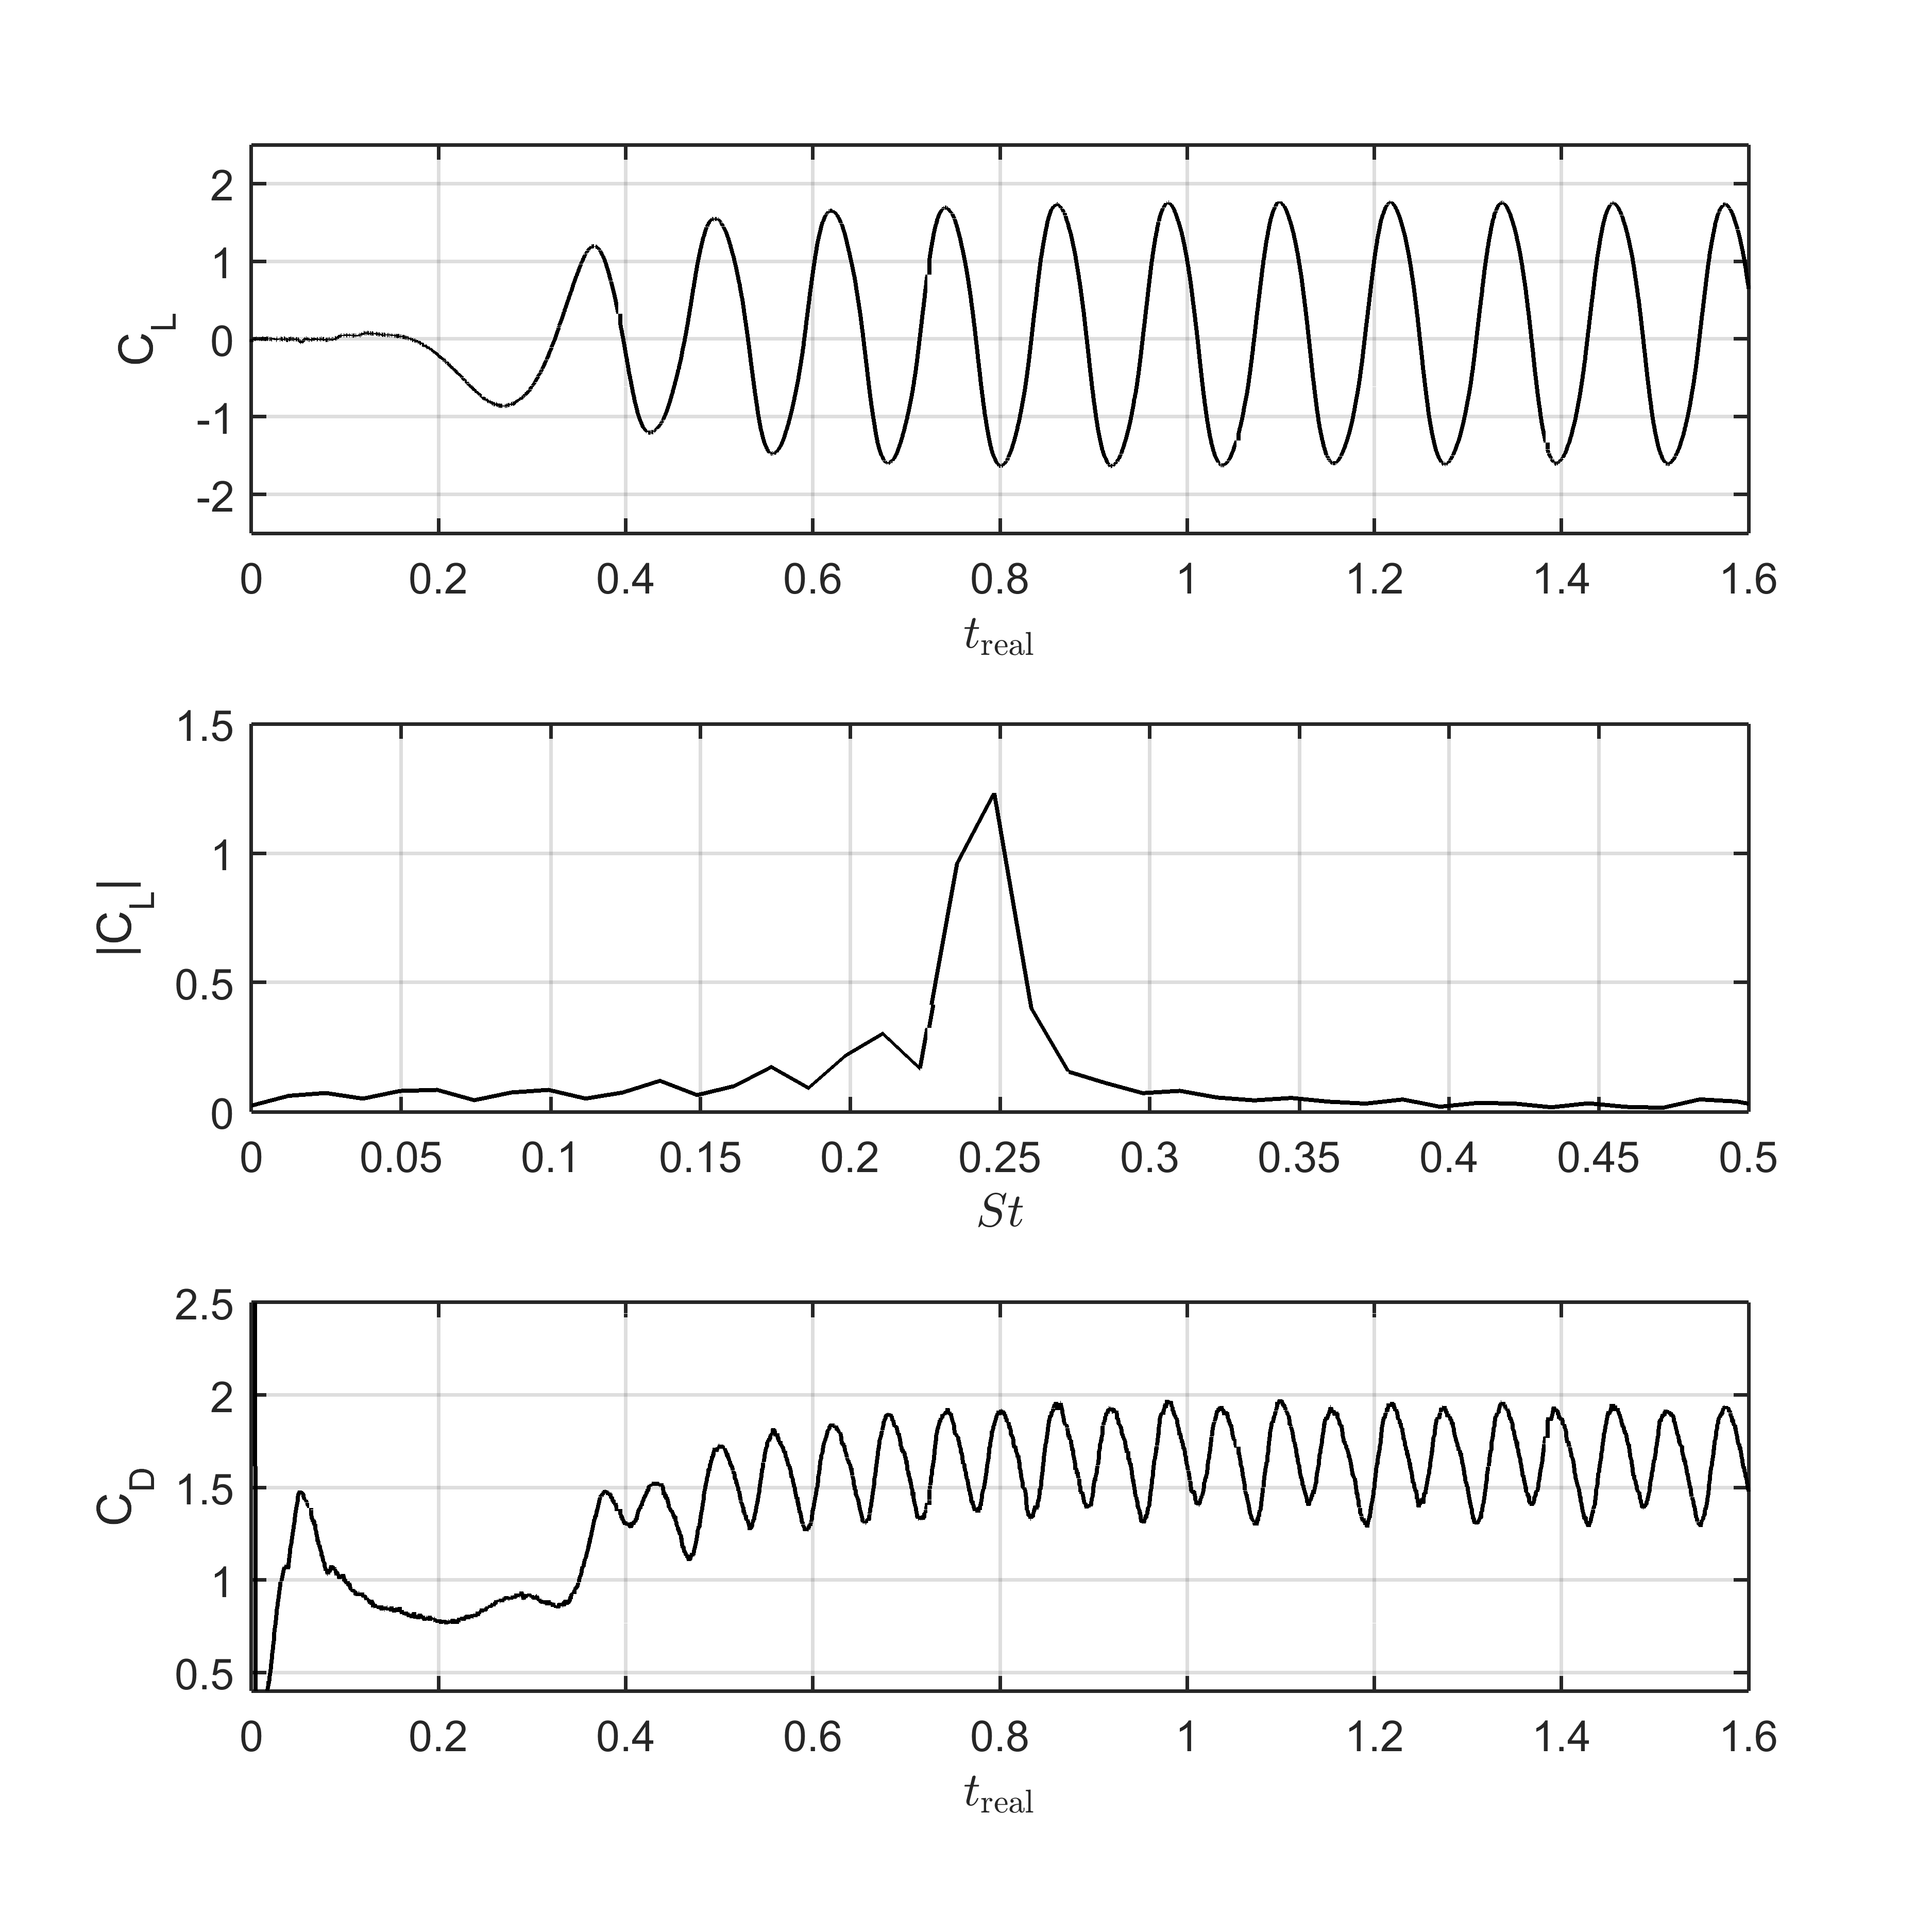
\includegraphics[width = 1\textwidth]{\lfsdir/figs/history_P5_filt_mesh4.png}
\caption{Case G in Table \ref{table:filteringEffect_simSummary} lift coefficient, \gls{st} power spectrum, and drag coefficient. Case is filtered and uses mesh \ref{fig:mesh_case_BDG} with $P=5$.} 
\label{fig:history_P5_filt_mesh4}
\end{figure}

\emph{Effect of changing the spatial order of accuracy while keeping the number of \gls{dof} constant.} Cases \hyperlink{caseA}{A} ($P=1$) and \hyperlink{caseB}{B} ($P=4$) keep close to the same number of \gls{dof}. Their lift coefficient power spectra show that the main vortex shedding frequencies are similar. Their drag coefficient figures reveal that \hyperlink{caseB}{Case B}, as expected, experiences less numerical dissipation; the initial vortices detach later than in \hyperlink{caseA}{Case A}. In addition, the drag coefficient plot in \hyperlink{caseB}{Case B} shows the presence of fairly small structures. \hyperlink{caseA}{Case A} seems to diffuse such structures. This effect can be seen in the corresponding videos as well.

\emph{Effect of changing the number of \gls{dof} while maintaining the spatial order of accuracy constant.} Cases \hyperlink{caseB}{B} and \hyperlink{caseC}{C} differ only in the mesh, \hyperlink{caseC}{Case C} has about half as many \gls{dof} as \hyperlink{caseB}{B}. Both cases have a peak in the lift coefficient power spectrum at \gls{st}$=0.17$. As can be seen in the videos and the drag coefficient plots, smaller structures are present in \hyperlink{caseB}{Case B}, however, \hyperlink{caseC}{Case C} still captures smaller structures than \hyperlink{caseA}{A} ($P=1$) while using half as many \gls{dof} and introduces less dissipation as demonstrated by \hyperlink{caseC}{Case C}'s delayed start of vortex shedding. The strength of the peak at \gls{st}$=0.17$ has decreased in \hyperlink{caseC}{Case C}. This points to the fact that higher dissipation increases the strength of shearing forces on the vortices, thus prompting earlier detachment and smaller lift coefficient oscillation amplitude.

\emph{Effect of using \gls{lfs} filters.}  Cases \hyperlink{caseB}{B} and \hyperlink{caseD}{D} differ only in the filtering. \hyperlink{caseD}{Case D} is filtered. The most salient effect of filtering is that the filtered solution starts shedding vortices earlier, sheds vortices periodically (as opposed to quasiperiodically), and very fine structures are almost non-existent. Indeed the flow looks like the case of \gls{re}$=100$ in Figure \ref{cylinder_3}, yet it predicts a higher mean drag coefficient. The power spectrum of the lift coefficient has very little energy at high values of \gls{st}. This is consistent with the desire of filtering specific frequencies from the simulation. Unfortunately the author could not find studies performed regarding the effect of artificial viscosity on the properties of chaotic flows. Nevertheless, the behavior observed in the filtered solution is consistent with what would be expected of a more viscous flow.

\emph{Effect of spatial order of accuracy on filtered simulations.} Cases \hyperlink{caseD}{D} and \hyperlink{caseG}{G} are both filtered and differ only in the spatial order of accuracy. The two simulations are nearly identical. This result is very encouraging: the filtering formulation maintains the spectral properties independent of the spatial order of accuracy. Recall that the filtering matrices are different for the different schemes. This means that the \gls{lfs} filters' spectral properties can be relied on when developing or using \gls{sgs} models.

\emph{Effect of the mesh on filtered simulations.} Cases \hyperlink{caseF}{F} and \hyperlink{caseG}{G} are both filtered and differ only in the mesh used. The peak \gls{st} number for the coarser grid, \hyperlink{caseF}{Case F}, is lower and its predicted average drag coefficient is lower. This result reflects the general high dependence of simulation results on the grid quality. The grid used in \hyperlink{caseF}{Case F} could not produce a stable unfiltered simulation result even with smaller time-steps. It is possible the shift in the drag coefficient is a reflection of the mesh's improper resolution. This shows that the \gls{lfs} filters could in some cases provide stability at the expense of accurate physics and confirms that \gls{lfs} filters de-couple stability from proper resolution.



% % % % % % % % % % % % % % % % % % % %  Conclusion
\subsubsection{Conclusion}
\label{sec:filterEffectsConclusion}
In the simulations summarized in Table \ref{table:filteringEffect_simSummary}, it was possible to isolate the effects of filtering on a \gls{re}$=3.9e3$, \gls{ma}$=0.1$ 2-D flow past a circular cylinder. The unfiltered solutions in different grids obtained with different spatial orders of accuracy displayed minor differences: all unfiltered flows showed quasiperiodic flow with a peak lift coefficient power at a frequency of \gls{st}$\approx 0.18$. All filtered solutions exhibited an apparent regime change: the flow became periodic and the peak lift coefficient power occurred at a higher frequency.

It could be surmised that the \gls{lfs} filters showed the following strengths:
\begin{enumerate}
\item The scales filtered by \gls{lfs} filters are relative to the element size and virtually independent of the order of the basis polynomials, this could be leveraged in the development of \gls{sgs} models. This was demonstrated by the extremely similar results of Cases \hyperlink{caseD}{D} and \hyperlink{caseG}{G}, which were performed in the same grid with different orders of accuracy.
\item \gls{lfs} filters de-couple stability from proper simulation resolution. This could be very helpful when performing \gls{les} of turbulent flows. If proper resolution were required for stability, such cases would need to have a resolution close to that of \gls{dns}.
\end{enumerate}

The following was identified as a potential drawback:
\begin{enumerate}
\item Application of \gls{lfs} filters in the entirety of the simulation can cause an artificial regime change consistent with what would be expected of increasing viscosity in the flow. This calls for a selective application of \gls{lfs} filters.
\item Because the spectral properties of \gls{lfs} filters scale with the element size, results of flows filtered throughout are grid dependent. Once again, the use of sensors could ameliorate this grid dependence.
\end{enumerate}




